\documentclass{egpubl}
\usepackage{egsgp15}
%\SpecialIssueSubmission
\SpecialIssuePaper
\electronicVersion
\PrintedOrElectronic
\usepackage{t1enc,dfadobe}
\usepackage{egweblnk}
\usepackage{cite}
\usepackage{amsmath}
\usepackage{microtype}

\title[Robust Articulated-ICP for Real-Time Hand Tracking] 
{Robust Articulated-ICP for Real-Time Hand Tracking}
%\author[Submission ID \#1027]{\Large Submission ID \#1027}
\author[Tagliasacchi et al.]{
Andrea Tagliasacchi$^{1*}$
\quad Matthias Schr\"oder$^{2*}$ % \thanks{Equal contributors.}
\quad Anastasia Tkach$^{1}$
\quad Sofien Bouaziz$^{1}$
\quad Mario Botsch$^{2}$
\quad Mark Pauly$^{1}$
\\
$^{1}$\'Ecole Polytechnique F\'ed\'erale de Lausanne (EPFL) \quad $^{2}$Bielefeld University \quad ($^*$equal contributors)}

%--- HACK: don't intent by default on new paragraph
\setlength{\parindent}{0pt}%

%-------------------------------------------------------------------------
\usepackage{overpic}
\usepackage{amssymb}
\usepackage{graphicx}
\usepackage{mathrsfs}
\usepackage{xcolor}
\usepackage{float} %< to define algorithms
\usepackage{anyfontsize} %< remove warnings
\usepackage{sidecap} %< caption on side

%%
%% general comments
%% 
% \usepackage{color}
\definecolor{turquoise}{cmyk}{0.65,0,0.1,0.3}
\definecolor{purple}{rgb}{0.65,0,0.65}
\definecolor{dark_green}{rgb}{0, 0.5, 0}
\definecolor{orange}{rgb}{0.8, 0.6, 0.2}
\definecolor{red}{rgb}{0.8, 0.2, 0.2}
\definecolor{blueish}{rgb}{0.0, 0.7, 1}
\definecolor{light_gray}{rgb}{0.7, 0.7, .7}
\definecolor{pink}{rgb}{1, 0, 1}
\definecolor{accent}{rgb}{179,81,109}
\definecolor{anagreen}{rgb}{.13,.627,.494}
\definecolor{anasalmon}{rgb}{.85,.604,.564}

%%
%% general comments
%% 
\newcommand{\hidden}[1]{{}} %< discards
\newcommand{\LEGACY}[1]{\textcolor{orange}{[LEGACY] #1}}
\newcommand{\todo}[1]{{\color{red}#1}}
\newcommand{\red}[1]{{\color{red}#1}}
\newcommand{\TODO}[1]{{\color{red}[TODO: #1]}}
\newcommand{\ADDRESSED}[1]{{}}
\newcommand{\copypaste}[1]{{#1}}
\newcommand{\revision}[1]{{#1}}
%\newcommand{\revision}[1]{{\color{red}#1}}
\newenvironment{DRAFT}{\colorlet{oldcolor}{.} \color{red}}{\color{oldcolor}}
% \newenvironment{edit}{\colorlet{oldcolor}{.} \color{dark_green}}{\color{oldcolor}}
\newenvironment{edit}{\colorlet{oldcolor}{.}}{\color{oldcolor}}

%%
%% personal comments
%% 
\newcommand{\AN}[1]{{\color{teal}[AN: #1]}} % anastasia 
\newcommand{\AT}[1]{{\color{pink}[AT: #1]}} % andrea
\newcommand{\MP}[1]{{\color{blueish}[MP: #1]}} % mark
\newcommand{\ER}[1]{{\color{orange}[ER: #1]}} % edo
\newcommand{\AF}[1]{{\color{blueish}[AF: #1]}} % andrew

%%
%% shortcut for references
%% 
\newcommand{\Fig}[1]{Fig.~\ref{fig:#1}}
\newcommand{\Figure}[1]{Figure~\ref{fig:#1}}
\newcommand{\Eq}[1]{Eq.~\ref{eq:#1}}
\newcommand{\Equation}[1]{Equation~\ref{eq:#1}}
\newcommand{\Optimization}[1]{Optimization~\ref{eq:#1}}
\newcommand{\Sec}[1]{Sec.~\ref{sec:#1}}
\newcommand{\Section}[1]{Section~\ref{sec:#1}}
\newcommand{\Appendix}[1]{Appendix~\ref{app:#1}}

%%
%% Inlined annotation of paragraph content
%% 
\newcommand{\brief}[1]{} % ONLY LATEX VISIBLE
% \newcommand{\brief}[1]{{\flushright\small{\vspace{-7pt}\color{light_gray} [\textbf{#1}]}\\}}

%%
%% SHOW PATH OF INSERTED IMAGES
%% 
\usepackage{currfile}
\newcommand{\putfilename}{}
% \newcommand{\putfilename}{ \put(-3,0){\rotatebox{90}{\color{red}\currfilename}}}

% Vertical text
\newcommand{\vertical}[1]{\rotatebox{90}{#1}}

%%
%% text layout
%%
% Insert whitespace at the end of a paragraph
\setlength{\parskip}{.5\baselineskip}%
% Don't intent by default on new paragraph
\setlength{\parindent}{0pt}%


%%
%% text layout
%%
\renewcommand{\paragraph}[1]{{\textbf{#1.}}}

%%
%% figure labels
%%
% \newcommand{\myfigurename}{\put(-4,0){\vertical{\todo{\currfiledir}}}}
\newcommand{\myfigurename}{}

%%
%% algorithm float (instead of table)
%%
\floatstyle{boxed}
\newfloat{algorithm}{t}{alg}
\floatname{algorithm}{Table}
\newcommand{\Tab}[1]{Tab.~\ref{tab:#1}}
\newcommand{\Table}[1]{Table~\ref{tab:#1}}
\begin{document}
\begin{figure}[H]
%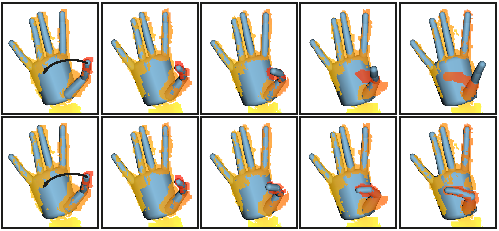
\includegraphics[width=\linewidth]{htrack/fig/teaser/composite.pdf}
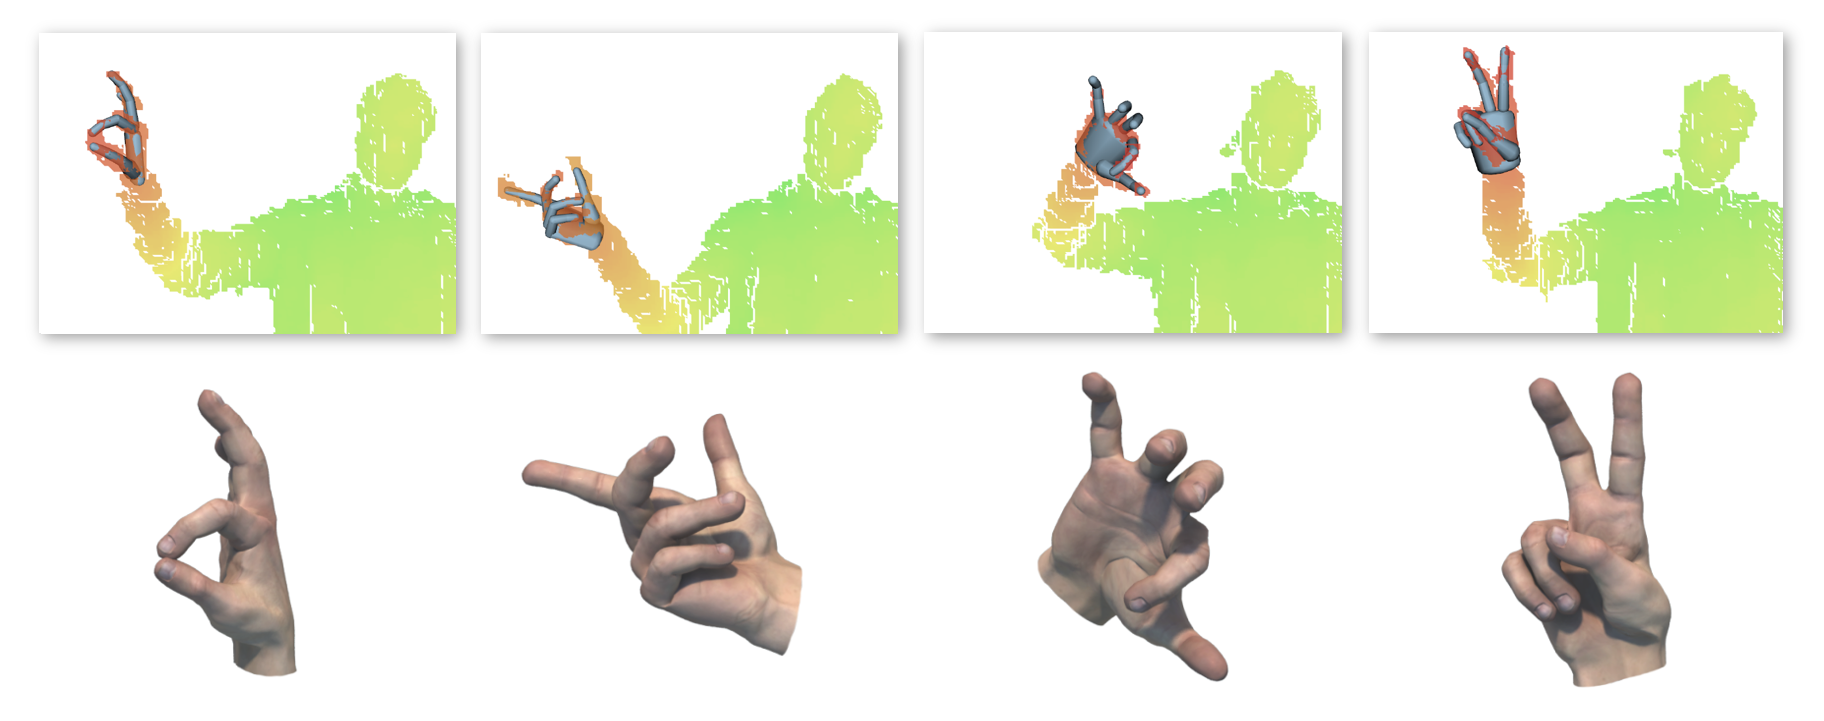
\includegraphics[width=\linewidth]{htrack/fig/teaser/teaser.png}
\centering
\caption{Our system tracks the motion of hands while remaining robust to fast motion, sensor imperfections and self-occlusions.}
% \label{fig:teaser}
\end{figure}
\maketitle
% !TEX root = ../hmodel.tex

This chapter is based on the following publication:

\begin{adjustwidth}{2.5em}{0pt}
\textsc{Tkach A., Pauly M., Tagliasacchi A.}: Sphere-meshes for real-time hand
modeling and tracking. \textit{In ACM Trans. Graph. (Proc. SIGGRAPH Asia) (2016)}.
\end{adjustwidth}

\section*{Abstract}

%--- Background
Modern systems for real-time hand tracking rely on a combination of discriminative and generative approaches to robustly recover hand poses. Generative approaches require the specification of a geometric model.
%--- Core point
In this chapter \todo{we propose a the use of sphere-meshes} as a novel geometric representation for real-time generative hand tracking. 
% 
\todo{How tightly this model fits a specific user heavily affects tracking precision.}
%--- Model Adaptation
We derive an optimization to non-rigidly deform a template model to fit the user data in a number of poses.
% 
%--- Performance
This optimization jointly captures the user's static and dynamic hand geometry, thus facilitating high-precision registration.
At the same time, the limited number of primitives in the \todo{tracking template} allows us to retain excellent \todo{computational} performance. We confirm this by embedding our models in an open source real-time registration algorithm to obtain a tracker steadily running at 60Hz.
%
%--- Why should I believe you?
We demonstrate the effectiveness of our solution by qualitatively and quantitatively evaluating tracking precision on a variety of complex motions. We show that the improved tracking accuracy at high frame-rate enables stable tracking of extended and complex motion sequences without the need for \todo{per-frame} re-initialization.
%
%--- Data release
To enable further research in the area of high-precision hand tracking, \todo{we publicly release source code and evaluation datasets.}
% together with the corresponding evaluation metrics.


\begin{figure}[t]
\centering
\begin{overpic} 
[width=\linewidth]
% [width=\linewidth,grid,tics=5]
{htrack/fig/data/composite.pdf}
\put(55,2){$\PointsSensorHtrack$}
\put(55,21){$\PointsSensorHtrack$}
\put(75,2){$\PointsSensorHtrack$}
\put(75,21){$\PointsSensorHtrack$}
\put(95,2){$\SilhoSensor$}
\put(95,21){$\SilhoSensor$}
\putfilename
\end{overpic}
\caption{
%
The two different sensors used in our experiments provide data with substantially different characteristics. Top: Intel's Creative Interactive Gesture camera (time of flight) provides a complete silhouette image \revision{$\SilhoSensor$}, but low quality depth measurements, resulting in severe noise in the point cloud \revision{$\PointsSensorHtrack$}. Bottom: Point clouds acquired by the PrimeSense camera (structured light) are much smoother, but the silhouette image can contain significant gaps.
\vspace{-.2in}
% 
} % caption
\label{fig:data}
\end{figure}

\section{Introduction} \label{sec:htrack-intro}

\brief{why is the problem important}
Tracking and animating humans in motion is a fundamental problem in computer graphics and computer vision. A particularly important question is how to accurately reconstruct the shape and articulation of human hands. Hand motion is a crucial component of non-verbal communication, plays an important role in the animation of humanoid avatars, and is central for numerous human-computer interfaces. 

Accurate realtime body tracking~\cite{shotton_cvpr11,wei_siga12} and face tracking~\cite{cao_sig14} systems have been recently proposed. Hand tracking is now gaining traction in the research community as a next natural step towards a complete system for online human communication in desktop environments~\cite{oiko2011hand,melax2013dynamics,sridhar2014anisotropic,schroder2014real,tompson2014real}.

Recent industrial trends in interaction systems for virtual environments have lead to the development of (closed source) software packages for the processing of RGBD data, like the Intel RealSense SDK, or purpose-designed hardware, like the Leap Motion and the Nimble sensors. 

\brief{why other approaches suck}

In this paper we introduce a system for \emph{realtime} hand tracking suitable for personal desktop environments. Our \emph{non-invasive} setup using a single commodity RGBD~sensor does not require the user to wear a glove or markers. 
Such single-camera acquisition is particularly advantageous as it is cheap, does not require any sensor calibration, and does not impede user movements. 

\brief{why is it still challenging}
Accurate hand tracking with a non-invasive sensing device in realtime is a challenging scientific problem. Human hands are highly articulated and therefore require models with sufficiently many degrees of freedom to adequately describe the corresponding motion space. Hand motion is often fast and exhibits intricate geometric configurations with complex contact patterns among fingers. 

With a single-camera RGBD setup, we are faced with incomplete data due to self-occlusions and high noise levels (see Figure~\ref{fig:data}).

Yet the simplicity of the hardware and the ease of deployment make this setup the most promising for consumer applications as evidenced by the recent proliferation of new consumer-level sensors.

To cope with the limited amount of available information, we employ an articulated template model as a geometric prior for shape completion and topology control. Our model does not only encode geometry, but also serves as a domain to represent information about \emph{plausible} hand poses and motions. This statistical information, built by analyzing a database of annotated poses, is directly embedded into the optimization, which
allows accurate tracking with a high number of degrees of freedom even in challenging scenarios.

\subsection*{Contributions}
% 
We present a complete system for realtime hand tracking using a single commodity RBGD input sensor. Our core technical contributions are:
% 
\begin{figure}[t]
\centering
\begin{overpic} 
[width=\linewidth]
% [width=\linewidth,grid,tics=5]
% {fig/handmodel/composite.png}
{htrack/fig/handmodel/composite.pdf}
\put(36,1){\small $\skelpoint_0$}
\put(38,9){\small $\skelpoint_1$}
\put(40,14){\small $\skelpoint_2$}
\put(42.5,19.5){\small $\skelpoint_3$}
\put(43.5,23){\small $\skelpoint_4$}
% Too cluttered if we put more!!!
\putfilename
\end{overpic}
\caption{ 
%
A visualization of the template hand model with the number and location of degrees of freedom of our optimization. From left to right: The cylinder model used for tracking, the skeleton, the BVH skeleton exported to Maya to drive the rendering, the rendered hand model. 
% Note the rig bones of fingertips are sligthly longer, as they extend until they touch the surface.
% \MP{Not sure if I understand the last sentence. Should we skip it?}
%\TODO{Replace (d) with posed rendered model.}
} % caption
\label{fig:handmodel}
\end{figure}


\begin {itemize}
\item \new{a novel articulated registration algorithm that efficiently integrates data and regularization priors into a \emph{unified} real-time solver; see \Section{optimization} and \Appendix{gpu},}
\item a combined 2D/3D registration method to align the 3D hand model to the acquired depth map and extracted silhouette image; see \Section{fitting},
\item a new way of computing data-to-model correspondences that accounts for occlusions and significantly improves the robustness of the tracking; see \Section{fitting},
\item a new regularization strategy that combines a statistical pose-space prior with kinematic and temporal priors to \new{simultaneously} ensure the inferred hand poses are plausible
%--- This is about the PCA-mean discussion we had in the rebuttal.
\new{and aid the algorithm in recovering from loss-of-tracking; see \Section{prior},}
\item \new{exposing an interesting relationship between the well known point-to-plane registration energy and Gauss-Newton linearization;  
see \Appendix{lindistance}.}
\end{itemize}

Another important contribution of our paper is that we fully disclose our source code\footnote{\url{https://github.com/OpenGP/htrack}}. To the best of our knowledge, no other freely available implementation is available, and we believe that publishing our code will not only ensure reproducibility of our results, but also facilitate future research in this domain.

\new{Note that there is a widespread belief \cite{wei_siga12,zhang_siga14,qian2014realtime} that ICP-like techniques are too local and prone to local minima to successfully deal with fast articulated motion. One of our contributions is to show this commonly held belief should be re-considered. We demonstrate that a regularized geometric registration approach in the spirit of ICP can achieve outstanding performance. We believe this will significantly impact future research in this domain, as it will allow further development of registration techniques for real-time tracking, in contraposition to commonly employed techniques from the vision community like  discriminative~\cite{tompson2014real} and PSO~\cite{qian2014realtime} methods.}

Our regularized geometric registration achieves robust, highly articulated hand tracking at up to 120 frames per second (fps).
%
We quantitatively and qualitatively compare the performance of our algorithm to recent appearance-based and model-based techniques (see \Section{eval}). These comparisons show a significant improvement in accuracy and robustness compared to the current state-of-the-art.

% !TEX root = ../hmodel.tex

% USE THIS? (good hand model key to high-quality in-hand scanning)
% http://files.is.tue.mpg.de/dtzionas/In-Hand-Scanning/

% I IGNORED THIS ONE, NOT ENOUGH DETAILS:
% Straka et al. \cite{straka2012simultaneous} also fit the template mesh with attached skeleton to 3D data. The model is deformed to explain the data while keeping the vertices attached to their corresponding bones. It is on clear whether the approach whether be able to handle a hand motion sequence, since the results are demonstrated on a full body model.

\begin{figure}[t]
\centering
\begin{overpic} 
[width=\linewidth]
% [width=\linewidth,grid,tics=10]
{\currfiledir/item.pdf}
\myfigurename{}
\put(1.5,86){\scriptsize \vertical{$mm$}}
\put(1.5,40){\scriptsize \vertical{$mm$}}
\put(83,1){\scriptsize $\sigma$}
\put(83,47){\scriptsize $\sigma$}
\end{overpic}
\caption{
% 
Mean and standard deviation for ground-truth calibration residuals as we vary the algorithm's initialization with a random perturbation of standard deviation $\sigma$. We evaluate the residuals on (top) synthetic depth maps, as well as (bottom) on the raw depth maps. (right) the exemplars drawn from the $\sigma=0.4$ perturbation used in the evaluation.
% 
}
\label{fig:synthetic}
\end{figure}

\section{Related Work}
\label{sec:related}

% \paragraph{Overkill} %< Instrumented + Multi-Camera
The simplest way of tracking a hand in motion is by instrumentation. We can place retro-reflective markers on the hand, wear a data glove with embedded abduction and flexion sensors~\cite{dipietro2008survey} or a colored glove~\cite{wang2009colorglove}. While effective, active instrumentation can be cumbersome as it requires lengthy preparation and/or calibration.
%\AnastasiaComment{We do we talk about these systems, they are from a different area and are solving completely different problems. If someone wrote related literature this way before, it does not mean that we have to do the same.}
Systems solely relying on computer vision (i.e.\ color cameras) are highly desirable, but pose estimation  relying on color information is extremely challenging~\cite{erol2007survey}: the complexity of hand motion, the large number of self-occlusions and rapidly changing backgrounds all contribute to their limited success. Multiple-camera acquisition can mitigate these challenges. In \cite{ballan2013salient}, the authors demonstrate high-quality tracking of two-hand and hand-object interactions. 
% REFUSE TO GIVE A CITE TO THIS GUY...
% , while \cite{wang2013physics} additionally considers the physics of motion interaction.
However, due to the substantial increase in data bandwidth, these algorithms do not scale to real-time performance.\todo{ A notable exception is the 10Hz system of  \cite{sridhar2013multicam}, but this acquisition setup also considers data from a depth sensor.} While providing accurate results, multi-camera rigs are  impractical for consumer-level applications. Therefore, we limit our attention to techniques relying on data from a \emph{single} depth camera; with a slight abuse of wording \todo{we refer to these systems as \emph{monocular} acquisition setups.}
% IGNORED THIS: place a camera directly on the user's wrist~\cite{kim2012digits}.

\paragraph{Hybrid = discriminative + generative}
% 
Pose estimation techniques can be grouped into \emph{discriminative} and \emph{generative} techniques, also known respectively as \emph{appearance-based} and \emph{model-based} approaches.
% Generative
Generative approaches fit a template through a temporal sequence of images~\cite{oiko2011hand,melax2013dynamics,schroder2014real,tagliasacchi2015robust}. Given an accurate template of the user being tracked, these methods can resolve highly accurate motion. As the optimization is initialized from the previous frame, tracking loss can occur, although simple geometric reinitialization heuristics can be employed to overcome this issue~\cite{melax2013dynamics,qian2014realtime}. 
% Discriminative
Conversely, discriminative methods estimate the pose by extracting features from each image independently by learning from a large dataset of annotated exemplars~\cite{keskin2012hand,tang2013real,tejani2014latent,sun2015cascaded}.
While discriminative methods avoid drift, they lack the accuracy of generative methods, and joint estimates often violate kinematic constraints, like consistent finger lengths and joint limits.
% Hybrid-1
State-of-the-art tracking performance is achieved by \emph{hybrid} algorithms that combine the two approaches. These algorithms estimate (potentially) multiple per-frame coarse poses leveraging discriminative frameworks, and then refine the alignment with a generative fitting~\cite{tompson2014real,qian2014realtime,sharp2015accurate}.
% Hybrid-2
Another class of hybrid algorithms introduce correspondences through a labeling obtained through a per-pixel forest  classifier~\cite{sridhar2015fast,fleishman2015icpik}.
% 
% What we (do not) cover?
Our literature review focuses on generative approaches, while we refer the reader to the very recent work by Taylor and colleagues \shortcite{taylor2016concerto} for a review of recent discriminative methods. Commercial systems for hand tracking like the \emph{NimbleVR}, the \emph{LeapMotion Orion} and the \emph{Intel Perceptual SDK} also exist, but it is difficult to consider them as the underlying technology is undisclosed.

\paragraph{Generative tracking models}
The capsule model originally proposed by~\cite{rehg1994tracking} has been adopted by a number of researchers \cite{oiko2011hand,schroder2014real,fleishman2015icpik,tagliasacchi2015robust}; see \Figure{handmodels}(a). Such a coarse representation is suitable to the task given the low signal-to-noise ratio in modern depth sensors, while its simplicity enables the efficient closed-form computation of alignment queries. Cylinders can also be approximated by a small set of disconnected spheres~\cite{qian2014realtime}, but this rough approximation is only sufficient for coarse-scale tracking. An alternative to cylinders and spheres is the use of isotropic~\cite{sridhar2013multicam,sridhar2015fast}, as well as anisotropic Gaussians~\cite{sridhar2014anisotropic}; see \Figure{handmodels}(b).
% while registration gradients can conveniently be computed in closed-form, the resulting tracking model is not appropriate for high-precision tracking.
% 
%
The use of surface meshes, while widespread in other domains (e.g.\ face tracking~\cite{bouaziz2013online} or offline registration~\cite{loper_eccv14}), has been limited to the visualization of tracking performance through skinned model animations~\cite{tompson2014real,schroder2014real}. Sharp et al.~\shortcite{sharp2015accurate} employed mesh models for tracking in a render-and-compare framework, while the very recent work of~\cite{taylor2016concerto} presents the first attempt towards a continuous registration framework for tracking hands with triangular meshes; see~\Figure{handmodels}(c).
%
Other variants of tracking models include the union of convex bodies from~\cite{melax2013dynamics}, \todo{a convolutional neural network capable of directly synthesizing hand depth images~\cite{oberweger2015feedback}}, and some \todo{initial attempts at tracking with implicit templates~\cite{fua2003soft}}.
% 
\todo{Our sphere-mesh model} offers accuracy comparable to triangle meshes used in \todo{recent hand} trackers, while retaining a compact representation for efficient correspondence queries and effective user adaptation.

\begin{figure}[t]
\centering
\begin{overpic} 
[width=\linewidth]
% [width=\linewidth,grid,tics=10]
{\currfiledir/item.pdf}
\myfigurename{}
\put(1.5,86){\scriptsize \vertical{$mm$}}
\put(1.5,40){\scriptsize \vertical{$mm$}}
\put(83,1){\scriptsize $\sigma$}
\put(83,47){\scriptsize $\sigma$}
\end{overpic}
\caption{
% 
Mean and standard deviation for ground-truth calibration residuals as we vary the algorithm's initialization with a random perturbation of standard deviation $\sigma$. We evaluate the residuals on (top) synthetic depth maps, as well as (bottom) on the raw depth maps. (right) the exemplars drawn from the $\sigma=0.4$ perturbation used in the evaluation.
% 
}
\label{fig:synthetic}
\end{figure}

\paragraph{Template calibration}
Albrecht et al.~\shortcite{albrecht2003construction} pioneered the creation of a realistic hand model (i.e. bones and muscles) by aligning a template mesh to data acquired by a laser-scanned plaster cast. Rhee et al.~\shortcite{rhee2006hand} use a simpler setup consisting of a single color image to identify approximate joint locations by localizing skin creases, and adapt a mesh template to conform to its silhouette. While these methods focus on a static template, in \cite{delagorce2011model} a model is roughly adapted to the user through simple bone scaling to produce the first \emph{animatable} template. 
% 
Calibration of a cylinder model through particle swarm has been investigated in~\cite{makris2015adapt}. \todo{Mesh calibration techniques were proposed in~\cite{taylor2014user} and extended in~\cite{khamis15learning}, which introduces compact and linear shape-spaces of human hand geometry.}
% 
The method in \cite{taylor2014user} shares some similarities with our work, where the model is adjusted to \emph{jointly} fit a set of depth frames, but with a fundamental difference in the way in which geometry is represented. \todo{Our sphere-mesh model} is \emph{naturally compact}, leading to straightforward calibration and tracking algorithms.

\paragraph{Implicit modeling}
Implicit sculpting tools have recently become a viable alternative to mesh or spline-based approaches for modeling complex geometries. This paradigm lies at the basis of the success of the \emph{PixoLogic ZBrush} product line. 
For articulated geometry, it is often convenient to first create a coarse geometric structure analogous to the one described in~\Equation{convsurf}, a process that \emph{PixoLogic} has re-branded as \emph{ZSphere{}} modeling; see \Figure{zsphere}. Editing the radii and centers of the sphere-mesh offers a \emph{natural} way of editing the model, making it easy for both humans and algorithms to calibrate.
%
Note that any geometric model can be approximated, to any desired precision, as a union of spheres~\cite{tagliasacchi2016skeletons}. 
However, by considering spheres that are linearly interpolated across edges, we can heavily reduce the required number of primitives. Following this principle, \cite{thiery2013sphere} recently investigated a method to automatically generate Sphere Meshes provided a  (static) input model. Extending this work, \cite{thiery2016spheremesh} proposed a method to fit a model to a sequence of dynamic meshes. 
% 
While seemingly related, our calibration optimization is solving a fundamentally different problem, as in our technique a template is fixed and provided in input.

% !TEX root = ../hmodel.tex

\begin{figure}[t]
\centering
\begin{overpic} 
[width=\linewidth]
% [width=\linewidth,grid,tics=10]
{\currfiledir/item.pdf}
\myfigurename{}
\put(1.5,86){\scriptsize \vertical{$mm$}}
\put(1.5,40){\scriptsize \vertical{$mm$}}
\put(83,1){\scriptsize $\sigma$}
\put(83,47){\scriptsize $\sigma$}
\end{overpic}
\caption{
% 
Mean and standard deviation for ground-truth calibration residuals as we vary the algorithm's initialization with a random perturbation of standard deviation $\sigma$. We evaluate the residuals on (top) synthetic depth maps, as well as (bottom) on the raw depth maps. (right) the exemplars drawn from the $\sigma=0.4$ perturbation used in the evaluation.
% 
}
\label{fig:synthetic}
\end{figure}

\section{Tracking}
\label{sec:tracking}
Given a calibrated hand model $\model$, our real-time tracking algorithm optimizes the 28 degrees of freedom $\parpose$ (i.e. joint angles) so that our hand model matches the sensor input data; the generation of a calibrated model $\model$ for a user is detailed in \Section{modeling}. Directly extending the open source \emph{htrack} framework of \cite{tagliasacchi2015robust}, we write our tracking optimization in Gauss-Newton/Levenberg-Marquardt form:
% 
\begin{eqnarray}
\parpose_t = \argmin_{\parpose}
\sum_{\mathcal{T} \in \termstrack} 
w_\mathcal{T} E_\mathcal{T}(\depth_t,\parpose,\parpose_{t-1})
\label{eq:htrack}
\end{eqnarray}
% 
where fitting energies are combined with a number of priors to regularize the solution and ensure the estimation of plausible poses. 

The energy terms $\termstrack$ in our optimization are:
% 
\begin{description}[labelsep=0em,labelwidth=.6in,labelindent=.25cm,itemsep=-.6em]
    \item[d2m]          each data point is explained by the model
    \item[m2d]          the model lies in the sensor visual-hull
    \item[pose]         hand poses sample a low-dimensional manifold
    \item[limits]       joint limits must be respected
    \item[collision]    fingers cannot interpenetrate
    \item[temporal]     the hand is moving smoothly in time
\end{description}
% 
We limit our discussion to the computational elements that need to be adapted to support sphere-meshes, while referring the reader to \cite{tagliasacchi2015robust} for other details.

\newpage
\paragraph{Hausdorff distance} 
% Generally speaking,
\todo{The similarity of two geometric models can be measured }by the symmetric Hausdorff distance $\metric_{X \leftrightarrow Y}$:
% 
\begin{eqnarray*}
\metric_{X \rightarrow Y} =& \max_{x \in X} \left[ \min_{y \in Y} \metric(x,y) \right] \\
\metric_{Y \rightarrow X} =& \max_{y \in Y} \left[ \min_{x \in X} \metric(x,y) \right] \\
\metric_{X \leftrightarrow Y} =& \max \{ d_{X \rightarrow Y}, \metric_{Y \rightarrow X} \}
\end{eqnarray*}
We therefore interpret our terms $E_{d2m}$ and $E_{m2d}$ as approximations to the asymmetric Hausdorff distances $\metric_{X \rightarrow Y}$ and $\metric_{Y \rightarrow X}$, where the difficult to differentiate \emph{max} operators are replaced by arithmetic means, and a robust $\ell_1$ distance is used~\cite{regcourse}.
% for $d(x,y)$.

\begin{figure}[t]
\centering
\begin{overpic} 
[width=\linewidth]
% [width=\linewidth,grid,tics=10]
{\currfiledir/item.pdf}
\myfigurename{}
\put(1.5,86){\scriptsize \vertical{$mm$}}
\put(1.5,40){\scriptsize \vertical{$mm$}}
\put(83,1){\scriptsize $\sigma$}
\put(83,47){\scriptsize $\sigma$}
\end{overpic}
\caption{
% 
Mean and standard deviation for ground-truth calibration residuals as we vary the algorithm's initialization with a random perturbation of standard deviation $\sigma$. We evaluate the residuals on (top) synthetic depth maps, as well as (bottom) on the raw depth maps. (right) the exemplars drawn from the $\sigma=0.4$ perturbation used in the evaluation.
% 
}
\label{fig:synthetic}
\end{figure}


\paragraph{Data $\rightarrow$ Model}
The first asymmetric distance minimizes the average closest point projection of each point $\point$ in the \todo{depth} frame $\depth$:
%
\begin{equation}
E_{d2m} = |\depth|^{-1} \sum_{\point \in \depth} \| \point - \proj_{\model(\pars)}(\point)\|_2^1
\label{eq:d2m}
\end{equation}
% 
Adapting this energy, as well as its derivatives, to sphere-meshes requires the specification of the projection operator $\proj_\model$ that is described in \Section{corresp}.

\paragraph{Model $\rightarrow$ Data}
The second asymmetric distance considers how our monocular acquisition system does not have a complete view of the model. While the 3D location is unknown, we can penalize the model from lying outside the sensor's \emph{visual hull}:
\begin{equation}
E_{m2d} = |\model(\pars)|^{-1} \int_{\pixel \in \model(\pars)} \| \pixel - \proj_{\depth}(\pixel)\|_2^1
\label{eq:m2d}
\end{equation}
In the equation above, \todo{the integral is discretized as a sum over the set of pixels obtained through rasterization; see ~\Section{rendering}. The rasterization renders the model to the image plane using the intrinsic and extrinsic parameters of the sensor's depth camera.}

% !TEX root = ../../thesis.tex


\begin{figure}[t]
\flushleft
\begin{overpic} 
[width=\linewidth]
% [width=.97\linewidth,grid,tics=5]
{htrack/fig/frontcorr/composite.pdf}
\put(98, 1){\tiny\rotatebox{90}{Converged}}
\put(98,18.7){\tiny\rotatebox{90}{First Iter.}}
\put(98,34.7){\tiny\rotatebox{90}{Initial.}}
\put(15,-3){\small(a)}
\put(43,-3){\small(b)}
\put(78,-3){\small(c)}
\put(9,32){\tiny$\PointsSensor$}
\put(25,43){\tiny$\handmodel$}
\put(17,37){\color{red}$\proj_\handmodel$}
\put(45,37){\color{red}$\proj_\handmodel$}
\put(73,37){\color{red}$\proj_{\visiblehand}$}
\putfilename
\end{overpic}
% \vspace{-.05in}
\caption{
% 
Illustration of correspondences computations. The circles represent cross-sections of the fingers, the small black dots are samples of the depth map. (a) A configuration that can be handled by standard closest point correspondences.
 (b) Closest point correspondences to the back of the cylinder model can cause the registration to fall into a local minimum. Note that simply pruning correspondences with back-pointing normals would not solve this issue, as no constraints would remain to pull the finger towards the data. (c) This problem is resolved by taking visibility into account, and computing closest points only to the portion $\visiblehand$ of $\handmodel$ facing the camera. % 
}
\label{fig:frontcorr}
\end{figure}

\section{Optimization}
\label{sec:optimization}
In this section we derive the objective functions of our model-based optimization method
and provide the rationales for our design choices. 
Let $\DataSensor$ be the sensor input data consisting of a 3D point cloud $\PointsSensorHtrack$ and 2D silhouette $\SilhoSensor$ (see \Figure{data}). Given a 3D hand model $\handmodel$ with joint parameters $\parsHtrack = \{ \theta_1, \theta_2,\hdots, \theta_{26} \}$, we aim at recovering the pose $\parsHtrack$ of the user's hand, matching the sensor input data $\DataSensor$. 
To achieve this goal, we solve the optimization 
problem
% 
%\begin{equation}
%\label{eq:tracking_optimization}
%\argmin_{\pars} E_{\text{fit}} + E_{\text{prior}},
%\end{equation}
%
\begin{equation}
\label{eq:tracking_optimization}
\min_{\parsHtrack} \:\: \underbrace{E_{\text{3D}} + E_{\text{2D}} \new{+ E_{\text{wrist}}}}_{\text{Fitting terms}} + \underbrace{E_{\text{pose}} + E_{\text{kin.}} + E_{\text{temporal}}}_{\text{Prior terms}},
\end{equation}
%
combining fitting terms that measure how well the hand parameters~$\parsHtrack$ represent the data frame $\DataSensor$, with prior terms that regularize the solution to ensure realistic hand poses. For brevity of notation we omit the arguments $\parsHtrack, \PointsSensorHtrack,\SilhoSensor$ of the energy terms. We first introduce the fitting terms and present our new solution to compute tracking correspondences. Then we discuss the prior terms and highlight their benefits in terms of tracking accuracy and robustness. 
%
More details on the  implementation of the optimization algorithm will be given in \Section{implementation} and the appendix.

\begin{figure}[t]
\centering
\begin{overpic} 
[width=\linewidth]
% [width=\linewidth,grid,tics=5]
{htrack/fig/occlusion/composite.pdf}
\put(22,-1){\small(a)}
\put(53,-1){\small(b)}
\put(85,-1){\small(c)}
\put(18,14){$c_1$}
\put(49,14){$c_1$}
\put(80,14){$c_1$}
\put(32,6){$c_2$}
\put(63,14){$c_2$}
\put(94,14){$c_2$}
\putfilename
\end{overpic}
\vspace{1em}
\caption{
% We illustrate the necessity to compute correspondences against
% 
Illustration of the impact of self-occlusion in correspondences computations. 
(a) The finger $c_2$ initially occluded by finger $c_1$ becomes visible, which causes new samples to appear. (b)  Closest correspondences to the portion of the model visible from the camera do not generate any constraints that pull $c_2$ toward its data samples. This is the approach in \protect\cite{wei_siga12}, where these erroneous matches are then simply pruned. (c) Our method also considers front-facing portions of the model that are occluded, allowing the geometry to correctly register.      
%
}
\label{fig:occlusion}
\end{figure}

\subsection{Fitting Energies}
\label{sec:fitting}


%\begin{figure}[t!]
\centering
\begin{overpic}
[width=\linewidth]
% [width=\linewidth,grid,tics=10]
{\currfiledir/item.pdf}
\put(1,30){{\small$\%$}}
\put(1,64){{\small$\%$}}
\put(93,37.5){{\small $E_{3D}$}}
\put(93,04.5){{\small $E_{2D}$}}
\end{overpic}
\caption{
% 
%
\todo{Each plot visualizes on the $y$ axis the portion of frames with a mean error metric below the value reported on the $x$ axis. We employ the \handyseq{teaser} sequence for this purpose. Curves closer to the top-left quadrant indicate better performance.}
% 
% Our method is quantitatively compared to the one of~\protect\cite{tagliasacchi2015robust} on the \handyseq{teaser} sequence.
% 
% 
}
\label{fig:comp2}
\end{figure}
\section{Calibration}
\label{sec:modeling}

\brief{Multi-Pose Data}
Our calibration procedure adapts our template model to a specific user from a set of $N$ 3D measurements $\{ \depth_1 \dots \depth_N \}$ of the user's hand in different poses. Multiple measurements are necessary, as it is not possible to understand the kinematic behavior by analyzing static geometry, and the redundancy of information improves fitting precision. Further, in  monocular acquisition this redundancy is essential, as single-view data is highly incomplete\todo{,} making the problem ill-posed. In our research we have experimented with datasets $\{\depth_n\}$ acquired via multi-view stereo (e.g. \emph{Agisoft Photoscan}), as well as a single RGBD sensor. 
Our calibration formulation can be employed for both acquisition modalities.
\todo{Dynamic reconstruction frameworks such as~\cite{newcombe2015dynfusion} or \cite{innmann2016volume} could also be used to generate a dynamic template mesh over which sphere-mesh decimation could be executed~\cite{thiery2016spheremesh}. 
However, as no public implementation is currently available, it is currently unclear how well these methods would cope with loop-closure for features as small as human fingers.}

\subsection*{Kinematics}
The rest-pose geometry of our model is fully specified by two matrices specifying the set of sphere positions $\restcenters$ and \todo{the set of} radii $\radii$. The geometry is then posed through the application of  kinematic chain transformations; see \Figure{posing}a. Given a point $\bar\pointHmodel$ on the model $\model$ at rest pose, its 3D position after posing can be computed by evaluating the expression:
% 
\begin{equation}
\pointHmodel = \left[ \Pi_{k \in K(\bar\pointHmodel)} \mathbf{\bar{T}}_k \mathbf{T}_k \mathbf{\bar{T}}_k^{-1} \right] \bar\pointHmodel
\label{eq:kinematic}
% we apply the posing transformation, then we re-apply the rest pose transformation to bring the point back in world coordinates
\end{equation}
%
where $\mathbf{T}_*$ are the \emph{pose} transformations parameterized by $\parpose$ and $\Pi$ left multiplies matrices by recursively traversing the kinematic chain $K$ of point $\bar\pointHmodel$ towards the root~\cite{buss2004introduction}. 
Each node $k$ of the kinematic chain is associated with an orthogonal frame $\mathbf{\bar{T}}_k$ according to which local transformations are specified. In most tracking systems, the frames $\mathbf{\bar{T}}_*$ are manually set by a 3D modeling artist and kept fixed across users. However, incorrectly specified kinematic frames can be highly detrimental to tracking quality; see \Figure{posing}(c,d) and \VideoKinematic{}. Therefore, in our formulation, the kinematic structure (i.e. the matrices $\mathbf{\bar{T}}_*$) is directly optimized from acquired data.

\begin{figure}[t!]
\centering
\begin{overpic} 
[width=\linewidth]
% [width=\linewidth,grid,tics=10]
{\currfiledir/item.pdf}
\put(93,37.5){{\small $E_{3D}$}}
\put(93,04.5){{\small $E_{2D}$}}
\put(1,30){{\small $\%$}}
\put(1,64){{\small $\%$}}
\end{overpic}
\caption{\todo{Calibrating progressively improves the 2D/3D tracking metrics, showing a remarkable improvement in tracking fidelity from~\protect\cite{tagliasacchi2015robust} to~\citeme{}.}}
\label{fig:calibeval}
\end{figure}
\begin{figure*}[h!]
\centering
\begin{overpic} 
[width=\linewidth]
% [width=\linewidth,grid,tics=10]
{hmodel/fig/calibration/item.pdf}
% \put(10,10){\todo{\Large Overlay Text}}
\end{overpic}
\caption{
% 
% 
A visualization of a few iterations of our calibration optimization procedure; see \VideoMVS{}. Each quadrant displays a data frame $\depth_n$, $n=1 \dots 4$. Within each quadrant we show three iterations of the optimization. The model being calibrated here is the one employed for real-time tracking in \VideoTeaser{}.
% 
% 
}
\label{fig:calibration}
\end{figure*}

% \newpage
\subsection*{Formulation}
Let $\parpose_n$ be the \emph{pose} parameters optimally aligning the rest-pose template to the data frame $\depth_n$, and $\parposture$ be the \emph{posture} parameters representing the transformations $\mathbf{\bar{T}}_*$ via Euler angles. 

For notational brevity, we also define $\parsHmodel_n=[\parpose_n, \parposture, \restcenters, \radii]$. Our calibration optimization can then be written as:
% 
\begin{eqnarray}
% \parposture, \centers, \radii =
\argmin_{\{\parsHmodel_n\}}
\sum_{n=1}^N 
\sum_{\mathcal{T} \in \termscalib} 
w_\mathcal{T} E_\mathcal{T}(\depth_n, \parsHmodel_n)
\label{eq:calibration}
\end{eqnarray}
% 
We employ a set of energies $\termscalib$ to account for different requirements. On one hand we want a model that is a good fit to the data; on the other, we seek a non-degenerate sphere-mesh template that has been piecewise-rigidly posed. The following calibration energies $\termscalib$ encode these requirements:
% 
\begin{description}[labelsep=0em,labelwidth=.4in,labelindent=1cm,itemsep=-.6em]
\item[d2m] data to model distance
\item[m2d] model to data distance
\item[rigid] elements are posed rigidly
\item[valid] elements should not degenerate
\end{description}
% 
To make this calibration more approachable numerically, we rewrite \Eq{calibration} as an alternating optimization problem:
% 
\begin{eqnarray}
% \restcenters, \radii, \posedcenters =
\argmin_{\posedcenters, \restcenters, \radii} &
\sum_{n=1}^N 
\sum_{\mathcal{T} \in \termscalib}
w_\mathcal{T} E_\mathcal{T}(\depth_n, \centers_n, \restcenters, \radii)
\label{eq:step1}
\\
% \parposes, \parposture =
\argmin_{\parposes,\parposture} &
\sum_{n=1}^N 
\sum_{\mathcal{T} \in \termscalib}
w_\mathcal{T} E_\mathcal{T}(\centers_n, \parsHmodel_n) 
\end{eqnarray}
% 
\todo{Our first step adjusts rest-pose sphere centers $\restcenters$ and radii $\radii$,} by allowing the model to fit to the data without any kinematic constraint beyond rigidity, and returning as a side product a set of \emph{per-frame} posed centers $\posedcenters$. 
Our second step takes the set $\posedcenters$ and projects it onto the manifold of kinematically plausible template deformations. 
This results in the optimization of the rotational components of rest-pose transformations $\mathbf{\bar{T}}_*$, as their translational components are simply derived from $\restcenters$.

\subsection*{Optimization}
The energies above are non-linear and non-convex, but can be optimized offline, as real-time tracking only necessitates a pre-calibrated model. For this reason, we conveniently employ the $lsqnonlin$ Matlab routine, which requires the gradients of our energies as well as an initialization point.
The initialization of $\restcenters$ is performed automatically by anisotropically scaling the vertices of a generic template to roughly fit the rest pose. The initial transformation frame rotations $\parposture$ are retrieved from the default template, while $\parposes$ are obtained by either aligning the scaled template to depth images, or by executing inverse kinematics on a few manually selected keypoints (multi-view stereo).
% 
% \AnastasiaComment{We should say that we use our tracking system with automatically scaled model to get the initial poses. Because the initial poses for calibration from sensor data are extremely close to the final ones. The model will not align to the from the rest pose, only tracking can do this. AT: I already wrote that, the sentence ``aligning the scaled template to the depth images''}
% 
Our (unoptimized) Matlab script calibrates the model within a few minutes for all our examples.


\subsection{Energies}
Our fitting energies are analogous to the ones used in tracking. They approximate the symmetric Hausdorff distance, but they are evaluated on \todo{a \emph{collection} of $N$ frames}:
% 
\begin{eqnarray}
E_{d2m} = 
\sum_{n=1}^N |\depth_n|^{-1} 
\sum_{\pointHmodel \in \depth_n} 
\| \pointHmodel - \proj_{\model(\parsHmodel_n)}(\pointHmodel)\|_2^1 \\
E_{m2d} = 
\sum_{n=1}^N |\model(\parsHmodel_n)|^{-1} 
\sum_{\pixelHmodel \in \model(\parsHmodel_n)} 
\| \pixelHmodel - \proj_{\depth_n}(\pixelHmodel)\|_2^1
\end{eqnarray}
% 
Note that the projection operator $\proj_{\depth_n}$ changes according to the type of input data. If a multi-view acquisition system is used to acquire a complete point cloud, then the projection operator fetches the closest point to $\pointHmodel$ in the point cloud of frame $\depth_n$. If $\depth_n$ is acquired through monocular acquisition, then $\proj_{\depth_n}$ computes the 2D projection to the image-space silhouette of the model.

\subsection*{Rigidity}
It is essential to estimate a \todo{single user template that, once articulated,} \emph{jointly} fits the set of data frames $\{ \depth_n \}$. For this purpose we require each posed model to be a piecewise-rigid articulation of our rest pose. \todo{This can be achieved by constraining each segment $\{ (\ballcenter_{n,i}, \ballcenter_{n,j})\:|\: ij \in \skeletonHmodel \}$ of $\centers_n$ to have the same length as the corresponding segment $(\bar\ballcenter_i, \bar\ballcenter_j)$ of the rest pose configuration $\restcenters$}:
% 
\begin{equation}
E_{\text{rigid}} = 
% \sum_{\ballcenter_{n,*} \in \centers_n}
\sum_{ij \in \skeletonHmodel} (\| \ballcenter_{n,i} - \ballcenter_{n,j} \| - \| \bar\ballcenter_i - \bar\ballcenter_j \|)^2
\end{equation}
% 
Note that only a subset of the edges of our control skeleton, as illustrated in \Figure{topology}, are required to satisfy this rigidity condition.

% \newpage
\subsection*{Validity}
The calibration optimization should avoid producing degenerate configurations \todo{in our \emph{rest pose} template $\restcenters$}. For example, a pill degenerates into a sphere when one of its balls is fully contained within  the volume of the other. Analogously, a wedge can degenerate into a pill or a sphere. We monitor validity by an indicator function $\chi(\bar\ball_i)$ that evaluates to one if $\bar\ball_i$ is degenerate and zero otherwise.
% 
\todo{We make a conservative choice and use $\chi(\bar\ball_i)$, which verifies whether $\bar\ballcenter_i$ is inside $\bar\oneelement \setminus \bar\ball_i$, the element obtained by removing a vertex, as well as all its adjacent edges, from $\bar\oneelement$.}
% 
This leads to the following \todo{conditional} penalty function:
% 
\begin{equation}
E_{\text{valid}} = 
\sum_{\bar\oneelement \in \restcenters}
\sum_{\bar\ball_i \in \bar\oneelement} 
\chi(\bar\ball_i) 
\| \bar\ballcenter_i - \proj_{\bar\oneelement \setminus \bar\ball_i}(\bar\ballcenter_i) \|_2^2
\end{equation}
% 
 


%Our fitting energy $E_{\text{fit}}$ captures the alignment of the hand model with the 3D point cloud and the 2D silhouette by combining two distinct energies
%% 
%\begin{equation}
%E_{\text{fit}} =  E_{\text{3D}} + E_{\text{2D}}.
%\label{eq:fitting}
%\end{equation}
%
%
% Our data fitting performs a joint 2D-3D op- timization. Our 3D alignment ensures that every point measured by the sensor Xs is sufficiently close to the tracked model M. Si- multaneously, as we cannot create such constraints for occluded portions of the hand, we optimize for a 2D registration that ensures the tracked M lies in the sensor visual hull Ss. O
%
%
% Our priors regularize the solution to ensure the recovered pose remains likely. We determined that retaining realistic hand postures is critical, as erroneous postures can result in establishing erroneous closest-point correspondences and cause catastrophic loss of tracking.
%


\subsection*{Point cloud alignment}
%The quality of the point cloud alignment is measured using $E_{\text{3D}}$. 
The term $E_{\text{3D}}$ models a 3D geometric registration in the spirit of ICP as
%. The energy is defined as
%
\begin{equation}
    E_{\text{3D}}  = \omegacloud \sum_{\pointHtrack \in \PointsSensorHtrack} \| \pointHtrack - \proj_{\handmodel(\parsHtrack)}(\pointHtrack,\parsHtrack) \|_2^1,
\label{eq:align3d}
\end{equation}
%
where $\|\cdot\|_2$ denotes the $\ell_2$ norm, $\pointHtrack$ represents a 3D point of $\PointsSensorHtrack$, and $\proj_{\handmodel(\parsHtrack)}(\pointHtrack,\parsHtrack)$ is the projection of $\pointHtrack$ onto the hand model $\handmodel$ with hand pose $\parsHtrack$. 
%This projection defines the correspondence of $\point$ on the model. For brevity of notation, we define this correspondence as $\mathbf{y} = \proj_{\handmodel}(\point,\pars)$.
%
 Note that we compute a sum of absolute values of the registration residuals, not their squares. This corresponds to a mixed $\ell_{2}/\ell_{1}$ norm of the stacked vector of the residuals. For 3D registration such a sparsity-inducing norm has been shown to be more resilient to noisy point clouds containing a certain amount of outliers
such as the ones produced by the Creative sensor (\Figure{data}). We refer to~\cite{Bouaziz_eg2014} for more details.

% \SB{not sure if we should say that here: As the 3D hand model is simply composed of cylinders, we compute the projections in close form ignoring back facing correspondences.}


\begin{figure}[t]
\centering
\flushleft
\begin{overpic} 
[width=.97\linewidth]
% [width=.97\linewidth,grid,tics=5]
{htrack/fig/occnrg/composite.pdf}
\put(100,2){\rotatebox{90}{\small{corresp. culling}}}
\put(100,24){\rotatebox{90}{\small{occlusion energy}}}
\putfilename
\end{overpic}
\vspace{1em}
\caption{
% 
Correspondence computations.
The top row shows the strategy 
% originally proposed for full-body tracking by \protect\cite{ganapathi_eccv12}
used in~\protect\cite{qian2014realtime} adapted to our gradient-based framework according to the formulation given in~\protect\cite{wei_siga12}. The bottom row shows the improved accuracy of our new approach.
% 
%The effect of replacing our view-dependent correspondence computation by an energy minimizing depth disparity~\protect\cite{wei_siga12} for portions of the model occluding the sensor data~\protect\cite{qian_cvpr14}. \MP{I don't understand the references. So the top row is Wei et al and the bottom row our method? Why refer to Qian?}
} % caption
\label{fig:occnrg}
\end{figure}

\subsection*{3D correspondences}
% The projection operators are now decoupled from the optimization and can be evaluated, rather than differentiated.
% The optimization problems in Step.1 can be solved in close form. The computation of 3D correspondences in \Equation{cp3d} can be performed either by exhaustively computing the distances to the underlying cylinder model, or by first rendering the point cloud with the same viewport of the sensor and then fetching closest points with a spatial data structure (kdtree or octree). \AT{Note that the first way of computing closest points is trivially parallelizable}
The 3D registration term involves computing the corresponding point  $\mathbf{y} = \proj_{\handmodel(\parsHtrack)}(\pointHtrack,\parsHtrack)$ on the cylinder model~$\handmodel$ for each sensor point $\pointHtrack \in \PointsSensorHtrack$. 
In contrast to standard closest point search, we define the correspondence $\mathbf{y}$  as the closest point on the \emph{front-facing} part $\visiblehand$ of $\handmodel$. This includes parts of the model that are oriented towards the camera but occluded by other parts. 
 In our experiments we learned that this seemingly simple extension proved absolutely essential to obtain high-quality tracking results.
 Only considering model points that are visible from the sensor viewpoint, i.e., matching to the rendered model, is not sufficient for handling occlusions or instances of disappearing and reappearing sensor data; see \Figure{frontcorr} and \Figure{occlusion}. 
 
To calculate $\mathbf{y}$, we first compute the closest points $\pointHtrack_\mathcal{C}$ of $\pointHtrack$ to each cylinder $\mathcal{C}\in\handmodel$. Recall that our hand model consists of sphere-capped cylinders so these closest points can be computed efficiently in closed form and in parallel for each $\pointHtrack \in \PointsSensorHtrack$.
We then identify back-facing points using the dot product of the cylinder surface normal $\mathbf{n}$ at $\pointHtrack_\mathcal{C}$ and the view ray vector $\mathbf{v}$. 
%
For efficiency reasons, we use a simplified orthographic camera model where the view rays are constant, i.e., $\mathbf{v} = [0~0~1]^T$. If a point on a cylinder is back-facing ($\mathbf{n}^T\mathbf{v}>0$), we project $\pointHtrack$ onto the cylinder's silhouette contour line from the camera perspective, whose normals are orthogonal to $\mathbf{v}$.

%We first compute the orthogonal projection of $\point$ onto the cylinder's center line segment. The point on the cylinder's surface is then found by moving back along the projection axis by the cylinder radius.


%As the sensor data only contains points that are visible from the camera's point of view, we only project to the parts of the cylinder that are front-facing with respect to the camera. This includes parts of the model that are oriented towards the camera but occluded by other parts of the model. Only considering model points that are visible from the sensor viewpoint, i.e., matching to the rendered model point cloud, is not sufficient for handling occlusions or instances of disappearing and reappearing sensor data (see \Figure{frontcorr} and \Figure{occlusion}). 



% 
% Conversely, to establish closest point correspondences to $\SilhoSensor$, we first compute its distance transform in linear time using~\cite{felzenszwalb_12} (1ms on a 320x240 image).
 
A different strategy to address visibility issues has been introduced \new{ in~\cite{qian2014realtime}. These methods} propose an energy that penalizes areas of the model falling in front of the data, which is then optimized using particle swarms. This energy can be integrated into our optimization following the formulation in \cite[Eq. 15]{wei_siga12}. However, such an energy is prone to create local minima in gradient-based optimization, as illustrated in \Figure{occnrg}. Here the thumb has difficulty entering the palm region, as it must occlude palm samples before reaching its target~configuration. Our correspondence search avoids such problems.
\new{Furthermore, note how~\cite{qian2014realtime} follows a \emph{hypothesize-and-test} paradigm where visibility constraints in the form of \emph{ray-casting} are easy to include. As discussed in  \cite{ganapathi_eccv12}, such constraints are much more difficult to include in iterative optimization techniques like ours. However, our front-facing correspondences computation provides a simple and elegant way to deal with such shortcomings.}


% takes the energy formulation of~, which was optimized by particle swarm optimization, and adapts it to our gradient-based formulation; see~.

% \MP{Does this make more sense? I would still like to give an explanation of what is happening here. People might not know Qian. Can we say in one sentence what the difference is?}

%\AT{this is a dangerous statement. We implement the energy proposed in \cite{qian_cvpr14} and then linearize it. It's the gradient of this energy that is f'd, but if you follow a particle swarm strategy it does work `ok'}, highlighting the improved tracking accuracy of our approach.

\begin{figure}[t]
\centering
\begin{overpic} 
[width=\linewidth]
% [width=\linewidth,grid,tics=5]
% {fig/push/composite.pdf} %f'd up transparency
{htrack/fig/push/composite.png}
\put(44,40){\small{$\SilhoSensor$}}
\put(44,18){\small{$\SilhoSensor$}}
\put(31.5,-2){\small{silhouette}}
\put(54.5,-2){\small{w/o silhouette}}
\put(79.5,-2){\small{w/ silhouette}}
\putfilename
\end{overpic}
\vspace{1em}
\caption{
% \todo{[push]}
Our 2D silhouette registration energy is essential to avoid tracking errors for occluded parts of the hand.
When no depth data is available for certain parts of the model, a plausible pose is inferred by ensuring that the model is contained within the sensor silhouette image $\SilhoSensor$.
% correctly track occluded geometry. In these scenarios, it is the lack of data of depth measurements in certain areas that drives pose inference - by ensuring our model is behind by the sensor silhouette $\SilhoSensor$.
}
\label{fig:push}
\end{figure}

\subsection*{Silhouette alignment}
The 3D alignment energy $E_{\text{3D}}$ robustly measures the distance between every point in the 3D point cloud~$\PointsSensorHtrack$ to the tracked model $\handmodel$. However, as hands are highly articulated, significant self-occlusions are common during tracking. Such self-occlusions are challenging, because occluded parts will not be constrained when only using a 3D alignment energy. For this reason, we use a 2D silhouette term $E_{\text{2D}}$ that models the  alignment of the 2D silhouette of our rendered hand model with the 2D silhouette extracted from the sensor data as 
%
%The second term $E_{\text{2D}}$ models a 2D geometric alignment in a similar manner than the $E_{\text{3D}}$ energy as
%
\begin{equation}
    E_{\text{2D}} = \omegasilhouette \sum_{\pixelHtrack \in \SilhoRender} \| \pixelHtrack - \proj_{\SilhoSensor}(\pixelHtrack,\parsHtrack) \|_2^2,
\label{eq:align2d}
\end{equation}
%
% where $\pixel$ is a 2D point of the rendered silhouette $\SilhoRender$, and $\proj_{\SilhoSensor}(\pixel,\pars)$ denotes the projection of $\pixel$ onto $\SilhoSensor$.
where $\pixelHtrack$ is a 2D point of the \emph{rendered} silhouette $\SilhoRender$, and $\proj_{\SilhoSensor}(\pixelHtrack,\parsHtrack)$ denotes the projection of $\pixelHtrack$ onto the \emph{sensor} silhouette $\SilhoSensor$.
%over the 2D silhouette extracted from the sensor data $\SilhoSensor$. 
% \SB{not sure if we should say that here: The projections are computed using the 2D distance transform of $\SilhoSensor$~\cite{....}.}
%
\Figure{push} shows why the silhouette term is crucial to avoid erroneous poses when parts of the model are occluded. 
Without the silhouette energy, the occluded fingers can mistakenly move to wrong locations, since they are not constrained by any samples in the depth map.







%\subsection{Correspondence Search}
%
%The 3D and 2D registration energies of Equations~\ref{eq:align3d} and~\ref{eq:align2d} require the computation of point correspondences from the data to the model. Our solution improves upon existing correspondence algorithms without compromising computational efficiency.
%
%



\subsection*{2D correspondences}
In \Equation{align2d}, we compute the silhouette image $\SilhoRender$ by first rendering the hand model $\handmodel$ from the viewpoint of the sensor, caching the bone identifier and the 3D location associated with each pixel in a texture.
% for the computation of the Jacobian in \Equation{jacobian2d} are cached in a texture. 
The projection function $\proj_{\SilhoSensor}(\pixelHtrack,\parsHtrack)$ to compute the
% For each pixels in $\SilhoRender$, we then identify
 closest corresponding point to the sensor silhouette is evaluated efficiently using the 2D distance transform of $\SilhoSensor$.
 We use the linear time algorithm of~\cite{felzenszwalb_12} and store at every pixel the index to the closest correspondence.
% To perform this task efficiently, we compute the 2D distance transform of $\SilhoSensor$ with a linear time algorithm~\cite{felzenszwalb_12}, i.e., at every pixel we store the distance transform value and the index to the closest correspondence.
% simple to evaluate in close form, as they simply require us to compute the closest point to either the tracking model $\handmodel$ or the silhouette of the sensor data $\SilhoSensor$.
% At each iteration we render $\handmodel$ from the viewpoint of the sensor
% We employ the color of each pixel to uniquely identify the originating bone. This information, as well as its 3D position are necessary to compute the gradient of~\Equation{align2d}.
% Step 2 can now be approached by Gauss-Newton optimization; we perform Taylor expansion of the residuals $\mathbf{r}$ of each energy term in \Equation{icp} as $\mathbf{r} \approx \mathbf{r}_0 + \J(\mathbf{r}_0) \delta\pars$, where $\J=\partial \mathbf{r} / \partial \pars$ is the Jacobian of the residuals, and then compute the optimal update as:
% %
% \begin{eqnarray}
% \delta\pars = (\J^t \J + \alpha \mathbf{I})^{-1} \J^t (\mathbf{r} - \mathbf{r_0})
% \label{eq:gaussnewton}
% \end{eqnarray}
% %
% A description of the rows that assemble $\J$, altogether with a description of the chain-rule derivatives is given in the appendix. In the equation above, the term weighted by $\alpha$ both ensures the system remains well conditioned and stabilizes the optimization by reducing the magnitude of the computed update.



% \brief{Convergence Speed}

\begin{figure}[t]
\centering
\begin{overpic} 
[width=\linewidth]
% [width=\linewidth,grid,tics=5]
{htrack/fig/shapespace/composite.pdf}
\putfilename
\end{overpic}
\caption{An illustration of the PCA pose-space used to regularize the optimization. Black dots denote the samples of the data base. 
High likelihood poses are located nearby the mean of the latent space (dark red). 
% Note how the eigenvalues of the PCA space skew the metric in such a way that certain axis offer a broader spectrum of likely poses.
The eigenvalues of the PCA define the metric in the low-dimensional space, skewing it in certain directions. Poses that, according to this metric, are far from the mean are likely to be unnatural and will be penalized in the optimization.
}
\label{fig:shapespace}
\end{figure}

\subsection*{Wrist alignment}
\new{The inclusion of the forearm for hand tracking has been shown beneficial in~\cite{melax2013dynamics}. Our wrist alignment energy encodes a much simplified notion of the forearm in the optimization that enforces the wrist joint to be located along its axis.}
\begin{equation}
    E_\text{wrist} = \omegawrist \| \proj_\text{2D}(\mathbf{k}_0(\parsHtrack)) - \proj_{\ell}(\mathbf{k}_0(\parsHtrack)) \|_2^2,
\end{equation}
\new{
Minimizing this energy helps preventing the hand from erroneously rotating/flipping during tracking; an occurrence of this can be observed at \VideoHtrackWrist \footnote{Please find the accompanying Video1 at \url{http://lgg.epfl.ch/publications/2015/Htrack_ICP/new_video.mp4}
.}.
% 
Here $\mathbf{k}_0$ is the 3D position of the wrist joint, and $\ell$ is the 2D line extracted by PCA of the 3D points associated with the wristband; see \Figure{wristband}. Note that $\proj_\text{2D}$ causes residuals to be minimized in screen-space, therefore the optimization of this energy will be analogous to the one of \Equation{align2d}. 
We optimize in screen space because, due to occlusion, we are only able to observe half of the wrist and this causes its axis to be shifted toward the camera.}

\begin{figure}[t]
\centering
\begin{overpic} 
[width=.8\linewidth]
% [width=.8\linewidth,grid,tics=5]
{htrack/fig/shapespaceproj/composite.pdf}
\put(36,45){$\parsHtrack$}
\put(26,31){$\tilde\parsHtrack$}
\put(26,23){$\boldsymbol{\mu}$}
\put(39,6){$\posespace$}
% \put(25,31){$\tilde\pars$}
\putfilename
\end{overpic}
\caption{
% 
An illustration of the energies involved in our pose-space prior. For illustration purposes the full dimensional parameter vector $\parsHtrack\in\mathbb{R}^3$, while latent space variable $\tilde\parsHtrack\in\mathbb{R}^2$.
% 
The PCA optimization in \protect\cite{schroder2014real} constrains the pose parameters $\parsHtrack$ to lie on the subspace~$\posespace$. Conversely, we penalize the distance of our pose from~$\posespace$~(\Equation{pcaproj}); simultaneously, we ensure our pose remains likely by preventing it from diverging from the mean of the distribution~(\Equation{pcareg}).
% 
% either limiting the freedom of motion of the hand.
% This reduces the freedom of motion, as only poses in the subspace
% This can result in erroneously recovered poses, as $\pars$ can
% 
}
\label{fig:shapespaceproj}
\end{figure}
\begin{figure}[b]
%\flushright
\begin{overpic} 
[width=.98\linewidth]
%[width=.98\linewidth,grid,tics=5]
{htrack/fig/pcaconv/composite_new.pdf}
\put(-1,38){\rotatebox{90}{\tiny{with pose prior}}}
\put(-1,65){\rotatebox{90}{\tiny{w/o pose prior}}}

\put(3.5,4){{\tiny{0}}}
\put(17.6,4){{\tiny{3}}}
\put(31.1,4){{\tiny{6}}}
\put(39.2,4){{\tiny{10}}}

\put(57.4,4){{\tiny{0}}}
\put(71,4){{\tiny{1}}}
\put(84.8,4){{\tiny{2}}}
\put(93.3,4){{\tiny{3}}}

\put(16,0){{\tiny{w/o data term}}}
\put(69,0){{\tiny{with data term}}}
\putfilename
\end{overpic}
\caption{Beyond favoring natural poses, the data prior term also positively affects convergence speed. Top: With the same number of iterations, only with activated data term does the model fully register to the scan. The illustration below shows how the same final state requires significantly fewer iterations with the data term.
}
\label{fig:pcaconv}
\end{figure}
\subsection{Prior Energies}
\label{sec:prior}
Minimizing the fitting energies alone easily leads to unrealistic or unlikely hand poses, due to the deficiencies in the input data caused by noise, occlusions, or motion blur. We therefore regularize the registration with data-driven, kinematic, and temporal priors to ensure that the recovered hand poses are plausible. Each of these terms plays a fundamental role in the stability of our tracking algorithm, as we illustrate below.

%% and is composed of three terms
%% 
%\begin{equation}
%E_{\text{prior}} = E_{\text{pose}} + E_{\text{kinematic}} + E_{\text{temporal}}.
%\label{eq:prior}
%\end{equation}
%%


%The $E_{\text{kinematic}}$ energy aims at generating a plausible hand posture by finding a hand pose respecting some kinematic constraints, i.e., angle bounds and the avoidance of self-collisions. The $E_{\text{temporal}}$ term enforces temporal smoothness to avoid jittering and in order to predict hand parameters in  case of missing data. Finally, to achieve a tracking that produces  postures realizable by a human hand we employ a data-driven energy $E_{\text{pose}}$. 


\subsection*{Pose Space Prior (data-driven)}
\begin{figure}[t]
\centering
\begin{overpic} 
[width=\linewidth]
% [width=\linewidth,grid,tics=5]
{htrack/fig/pca/composite.pdf}
\put(30,-2.5){\small{depth image}}
\put(55,-2.5){\small{without PCA}}
\put(81,-2.5){\small{with PCA}}
\putfilename
\end{overpic}
\vspace{1em}
\caption{
% 
Our pose-space regularization using a PCA prior ensures that a meaningful pose is recovered even when significant holes occur in the input data.
}
\label{fig:pca}
\end{figure}

The complex and highly coupled articulation of human hands is difficult to model directly with geometric or physical constraints. Instead, we use a publicly available database of recorded hand poses~\cite{schroder2014real} to create a data-driven prior $E_{\text{pose}}$ that encodes this coupling.
% To achieve a tracking that produces hand postures which are realizable by a human hand (e.g. we cannot bend a finger on itself), we employ a data-driven regularizer. As a simple example, it is difficult to bend the \emph{distal phalanx} without simultaneously bending the \emph{proximal phalanx}.
We construct a low-dimensional subspace of plausible poses by performing dimensionality reduction using PCA (see \Figure{shapespace}). 
% 
%\begin{eqnarray}
%E_{\text{pose}} = E_{\text{projection}} + E_{\text{mean}}.
%\end{eqnarray}
%
We enforce the hand parameters~$\parsHtrack$ to lie close to this low-dimensional linear subspace using a 
 data term
$E_{\text{pose}} = E_{\text{projection}} + E_{\text{mean}}$.
%
To define the data term, we introduce auxiliary variables $\parssub$, i.e, the PCA weights, representing the (not necessarily orthogonal) projection of the hand pose $\parsHtrack$ onto the subspace; see \Figure{shapespaceproj}.
%\MB{If $\parssub$ is the projection of $\pars$ to the PCA space, then it is \emph{not} an auxiliary variable, since it is not free to be chosen differently. It is fully defined by $\pars$ and the PCA matrix $P$ as $\parssub = P P^T (\pars-\boldsymbol{\mu}$. You seem to really use it as an auxiliary variable, but then the above statement is wrong, and I don't see why you have to add the extra variables.}
The projection energy  measures the distance between the hand parameters and the linear subspace as
% 
\begin{eqnarray}
E_{\text{projection}}  = \omegapcaproj \|(\parsHtrack - \boldsymbol{\mu}) - \proj_\posespace \parssub \|_2^2,   
\label{eq:pcaproj}
\end{eqnarray}
% 
where $\boldsymbol{\mu}$ is the PCA mean. The matrix $\proj_\posespace$, i.e., the PCA basis,
%\MB{The PCA matrix (let's call it $P$), with the PCA basis vectors in its columns, is \emph{not} a projection. The projection matrix onto the PCA subspace is $PP^T$.}
reconstructs the hand posture from the low-dimensional space. 
%\MB{Why not simply measure the distance of $\pars$ from the subspace? This should by $\| (I-PP^T)(\theta-\mu) \|$. For \Eq{pcaproj} there's no need for an extra $\parssub$. }
To avoid unlikely hand poses in the subspace, we regularize the PCA weights $\parssub$ using an energy
% 
\begin{eqnarray}
E_{\text{mean}} = \omegapcareg \|\boldsymbol{\Sigma} \parssub \|_2^2. 
\label{eq:pcareg}
\end{eqnarray}
% 
$\boldsymbol{\Sigma}$ is a diagonal matrix containing the inverse of the standard deviation of the PCA basis.
Our tracking optimization is modified to consider the pose space by introducing the auxiliary variable $\tilde\parsHtrack$ and then jointly minimizing over $\parsHtrack$ and $\tilde\parsHtrack$. \new{The difference between our approach and optimizing directly in the subspace is further discussed in~\Appendix{pca}}.
% 
\new{Note how the regularization energy in \Equation{pcareg} helps the tracking system recover from tracking failures. When no sensor constraints are imposed on the model, the optimization will attempt to push the pose towards the mean -- a statistically likely pose from which tracking recovery is highly effective.}

\Figure{pca} illustrates how the PCA data prior improves tracking by avoiding unlikely poses, in particular when the input data is incomplete.
We found that even when data  coverage is sufficient to recover the correct pose, the data term improves the convergence of the optimization as illustrated in \Figure{pcaconv}.
% 
\Figure{pcafail} shows how our regularized projective PCA formulation outperforms the direct subspace optimization proposed in previous work.




% \todo{Explain why this is better than measuring the distance to the projection.}

\subsection*{Kinematic Prior}
The PCA data term is a computationally efficient way of approximating the space of plausible hand poses.
However, the PCA model alone cannot guarantee that the recovered pose is realistic. In particular, since the PCA is symmetric around the mean, fingers bending backwards beyond the physically realistic joint angle limits are not penalized by the data prior. Similarly, the PCA model is not descriptive enough to avoid self-intersections of fingers. These two aspects are addressed by the kinematic prior $E_{\text{kinematic}} = E_{\text{collision}} + E_{\text{bounds}}$.
%
%\begin{eqnarray}
%E_{\text{kinematic}} = E_{\text{collision}} + E_{\text{bounds}}.
%\label{eq:kinematic}
%\end{eqnarray}
%
Under the simplifying assumption of a cylinder model, we can define an energy $E_{\text{collision}}$ that accounts for the inter-penetration between each pair of (sphere-capped) cylinders:
% 
\begin{equation}
    E_{\text{collision}} = \omegacollision \sum_{\{i,j\}} {\chi(i,j)}(d(\cyl_i, \cyl_j) - r)^2,
\end{equation} 
%
where the function $d(\cdot,\cdot)$ measures the Euclidean distance between the cylinders axes $\cyl_i$ and $\cyl_j$, and $r$ is the sum of the cylinder radii. ${\chi(i,j)}$ is an indicator function that evaluates to one if the cylinders $i$ and $j$ are colliding, and to zero otherwise.
% \MB{I don't like the $\chi$, it messes up the equation. Why not use truncated powers, as people playing with compact kernels use: $(r-d(c_i,c_j))_+^2$, where $(x)_+^2$ is $x^2$ for $x>0$ and $0$ otherwise. It's clear what you want to model, but the $\chi$ just makes the equation (appear) unnecessarily complicated.}
The top row of \Figure{posepriors} shows how this term avoids interpenetrations of the fingers.
% \MP{Should add a figure that shows this effect} DONE
% 

\begin{figure}[t]
\centering
\begin{overpic} 
[width=\linewidth]
% [width=\linewidth,grid,tics=5]
{htrack/fig/pcafail/composite.pdf}
\renewcommand{\yoff}{-4}
\put(05,\yoff){\small$89\%$, \#PCA=4}
\put(30,\yoff){\small$96\%$, \#PCA=6}
\put(54,\yoff){\small$99\%$, \#PCA=9}
\put(79,\yoff){\small$79\%$, \#PCA=2}
\renewcommand{\yoff}{-8}
\put(08,\yoff){\small$\omegapcaproj=10^8$}
\put(33,\yoff){\small$\omegapcaproj=10^8$}
\put(57,\yoff){\small$\omegapcaproj=10^8$}
\put(82,\yoff){\small$\omegapcaproj=10^2$}
\putfilename
\end{overpic}
\vspace{2em} % leave enough space for overpic
\caption{
%
Optimizing directly in the PCA subspace~\protect\cite{schroder2014real} can lead to inferior registration accuracy.
We replicate this behavior by setting $\omegapcaproj$ in Equation~\ref{eq:pcaproj} to a large value. Even when increasing the number of PCA bases to cover $99\%$ of the variance in the database, the model remains too stiff to conform well to the input. Our approach  is able to recover the correct hand pose by optimizing for projection distances even with a very limited number of bases (right).}
\label{fig:pcafail}
\end{figure}

% by optimizing for projection distance (\Equation{pcaproj}) we can
% 
% We directly compare our method to the one in  by varying the number of PCA bases. Note how are technique is capable to fit well to the data with a very limited number of PCA bases.
% 
% (bottom) To decouple improvements due to our fitting energies, we realize the subspace optimization of \protect\cite{schroeder_icra14} by setting the latent projection weight $\omegapcaproj=10^{8}$.

%computed in close form as the shortest segment between the two cylinders axes
% \SB{To prevent fingers inter-penetrating each other during tracking we instantiate collision constraints. Similarly to \cite{oiko_?}, to retain real-time performance, we only instantiate constraints between nearby finger segments.}
To prevent the hand from reaching an impossible posture by overbending the joints, we limit the joint angles of the hand model:
\begin{equation}
   E_{\text{bounds}} = \omegabounds \sum_{\theta_i \in \parsHtrack}
        \underline{\chi}(i)(\theta_i - \underline{\theta}_i)^2
            +
        \overline{\chi}(i)(\theta_i - \overline{\theta}_i)^2,
        \label{eq:bound}
\end{equation}
%
% \MB{Same suggestion here: Replace $\chi$ by a truncated power, then you don't need to introduce two new $\chi$s}
where each hand joint is associated with conservative bounds $\left[ \underline{\theta}_i,\overline{\theta}_i\right]$. For the bounds, we use the values experimentally determined by \cite{chan1995weighted}.  {$\underline{\chi}(i)$} and {$\overline{\chi}(i)$} are indicator functions. {$\underline{\chi}(i)$} evaluates to one if $\theta_i < \underline{\theta}_i$, and to zero otherwise. $\overline{\chi}(i)$ is equal to one if $\theta_i > \overline{\theta}_i$, and  zero otherwise.
% \AT{should we say something about the fact that they lose meaning unless the palm is aligned correctly? This would make}
The bottom row of \Figure{posepriors} illustrates the effect of the joint angle bounds.

\begin{figure}[t]
\flushleft
\begin{overpic} 
[width=.95\linewidth]
% [width=.95\linewidth,grid,tics=5]
{htrack/fig/posepriors/composite.pdf}
\put(100,36.5){\rotatebox{90}{\tiny{collision}}}
\put(100,7){\rotatebox{90}{\tiny{joint limits}}}
\put(9,-2){\tiny{color}}
\put(34,-2){\tiny{depth}}
\put(57,-2){\tiny{disabled}}
\put(82.5,-2){\tiny{enabled}}
\putfilename
\end{overpic}
\vspace{0pt}
\caption{Kinematic priors augment the data prior to account for inconsistencies in the pose space. The collision term avoids self-collisions (top row), while the term for joint angle bounds avoids overbending of the finger joints.
% (top) Our latent pose space can contain poses with self-intersecting geometry. The collision energy prevents our tracking model from falling in these strong registration local minima. (bottom) As we only penalize the distance from the mean pose, given enough fitting constraints, our tracked model can assume unlikely poses. Joint bounds give further structure to the latent space by preventing the creation of unrealizable poses; also see \Figure{shapespaceproj}}.
}
\label{fig:posepriors}
\end{figure}



\begin{figure}[t]
\centering
\begin{overpic} 
[width=\linewidth]
% [width=\linewidth,grid,tics=5]
{htrack/fig/temporal/composite.pdf}
\put(1.2, 5){\small\rotatebox{90}{w/ temporal}}
\put(1.2, 25.5){\small\rotatebox{90}{w/o temporal}}
\put(22, 42){\small{50}}
\put(40, 42){\small{100}}
\put(59, 42){\small{150}}
\put(78, 42){\small{200}}
% labels
\put(14,-2.5){\small(a)}
\put(38,-2.5){\small(b)}
\put(62,-2.5){\small(c)}
\put(86,-2.5){\small(d)}
% plot labels
\put(42.75,69){\small(a)}
\put(47.4, 69){\small(b)}
\put(50.6, 69){\small(c)}
\put(55.5, 69){\small(d)}
% Y
\put(-.5, 56){\small{\rotatebox{0}{ 50}}}
\put(-.5, 68){\small{\rotatebox{0}{100}}}
\put(2, 72){\small{y}}
\putfilename
\end{overpic}
\vspace{1em}
\caption{The effect of the temporal prior. The graph shows the trajectory of the $y$-coordinate of the  fingertip over time as the index finger is bend up and down repeatedly. The temporal prior reduces jitter, but also helps avoiding tracking artifacts that arise when fragments of data pop in and out of view. %see also \Figure{data}-(bottom).
} % caption
\label{fig:temporal}
\end{figure}
\subsection*{Temporal Prior}

A common problem in particular with appearance-based methods are small-scale temporal oscillations that cause the tracked hand to jitter. A standard way to enforce temporal smoothness is to penalize the change of model parameters~$\parsHtrack$ through time, for example, by penalizing a quadratic energy accounting for velocity $\|\dot \parsHtrack\|^2$ and acceleration $\|\ddot \parsHtrack\|^2$~\cite{wei_siga12}. 
% 
% \MP{Please verify that it's ok to cite them here} \AT{it's correct}
% 
However, if we consider a perturbation of the same magnitude, it would have a much greater effect if applied at the root, e.g., global rotation, than if applied to an element further down the kinematic tree, e.g., the last phalanx of a finger. 
%\AT{we should say that this was what was done in ?} \MP{What did they do, our method, or the standard approach described above?}
%\AT{they do the standard approach. Never seen what we do around...}
% \todo{Also, it is not intuitive to understand how to tune its weighting parameter... compare angles with translations, and then to other energies... little meaning!!}
Therefore, we propose a solution that measures the velocity and acceleration of a set of points attached to the kinematic chain. We consider the motion of vertices $\skelpoint$ of the kinematic chain $\mathcal{K}$ (\Figure{handmodel}) and build an energy penalizing the velocity and acceleration of these points:
% \MB{I would call the vertices $\skelpoint_i$ to match the figure}
\begin{eqnarray}
    E_{\text{temporal}} = \omegatemporalst \sum_{\skelpoint_i \in \mathcal{K}} \| \dot \skelpoint(\parsHtrack) \|_2^2 + \omegatemporalnd \sum_{\skelpoint_i \in \mathcal{K}} \| \ddot \skelpoint(\parsHtrack) \|_2^2.
\end{eqnarray}
%
% \MB{Mention how you compute the time-derivatives.}
\Figure{temporal} illustrates how the temporal prior reduces jitter and improves the overall robustness of the tracking; see also \VideoHtrackTemporal.

% !TEX root = ../htrack.tex
% \newpage



\section{Implementation}
\label{sec:implementation}
%\input{htrack/fig/constraints.tex}

%-------------------------------------------------------------------------------
%-------------------------------------------------------------------------------
% \subsection{Solver }
%-------------------------------------------------------------------------------
%-------------------------------------------------------------------------------

In this section we provide more details on the implementation of our optimization algorithm. The derivation of the necessary gradients and Jacobians is given in the appendix.

\paragraph*{Optimization.} The optimization of the tracking energy of \Equation{tracking_optimization} over the pose $\pars$ 
%\begin{equation}
%\label{eq:final_optimization}
%\argmin_{\pars, \parssub} E_{\text{fit}} + E_{\text{prior}}
%\end{equation}
is performed by solving the non-linear least squares problem with a Levenberg-Marquardt approach. 
% \MB{Do you really use Levenberg-Marquardt? Why? In all comparisons I did it was slower than Gauss-Newton. The theoretical advantage of LM is that it is has a larger region fo convergence, but that (a) comes at a price and (b) should not be our problem due to small frame-to-frame changes. How do you adapt the LM-parameter that blends between Newton-step and gradient-step?}
The assumption is that a current estimate of $\pars$ is known from which we then compute an update. More specifically, the high acquisition speed of the sensing device allows us to employ the optimized parameters from the previous time frame as the starting estimate. We then iteratively approximate the energy terms using Taylor expansion and solve a linear system to get the update $\delta\pars$ at each iteration (see appendix).
% A detailed description of the optimization is given in Appendix~\ref{sec:app} and \Appendix{opt}. 
As our algorithm achieves 60 fps tracking, the previously reconstructed pose is of sufficiently high quality allowing our solve to converge within seven iterations.

\begin{figure}[t]
\centering
\begin{overpic} 
[width=\linewidth]
% [width=\linewidth,grid,tics=5]
{htrack/fig/rigid/composite.pdf}
\putfilename
\end{overpic}
\caption{
%
% \todo{[rigid]} 
% 
During fast motion, optimizing directly for a fully articulated hand can lead to incorrect correspondences and cause loss of tracking (middle row). By compensating for the rigid motion ahead of solving for joint angles, our system can better capture fast movements (bottom row).
% 
}
\label{fig:rigid}
\end{figure}

\paragraph*{Initialization.} As a user enters the scene our method is initialized by the fingertip detection and fitting from~\cite{qian_cvpr14}.
Other appearance-based methods could be used for initialization as well \cite{tompson_tog14}. We also re-initialize the tracking in case a severe tracking failure is detected using the method of \cite{wei_siga12}. Such re-initialization occurs rarely (e.g.\ less than $0.5\%$ of the frames in the sequence of \Figure{tompson}).


\paragraph*{Rigid bias.}
To improve the convergence of our solver in case of fast motion, we first perform the optimization in \Equation{tracking_optimization} 
% \MB{use brackets for referencing equations} 
for the rigid motion only by optimizing for the root of the kinematic chain. As shown in \Figure{rigid}, optimizing first for the rigid motion prior to the full pose estimation leads to improved robustness of the tracking.

 



% \AT{mention rigid iteration, perhaps show it in the analysis}
% as $\mathbf{r} \approx \mathbf{r}_0 + \J(\mathbf{r}_0) \delta\pars$, where $\J=\partial \mathbf{r} / \partial \pars$ is the Jacobian of the residuals, and then compute the optimal update as:
% %
% \begin{eqnarray}
% \delta\pars = (\J^T \J + \alpha \mathbf{I})^{-1} \J^T \mathbf{r_0}
% \label{eq:gaussnewton}
% \end{eqnarray}
% %
% A description of the rows that assemble $\J$, altogether with a description of the chain-rule derivatives is given in the appendix. The identity matrix $\mathbf{I}$ weighted by $\alpha$ ensures that the system remains well conditioned and stabilizes the optimization by reducing the magnitude of the computed update.

% this assumes the device's acquisition speed is sufficiently high to capture the hand movement
% Note that in \Equation{tracking_optimization},  $\proj_{\handmodel}(\point,\pars)$ and $\proj_{\SilhoSensor}(\pixel,\pars)$ are not differentiable \SB{that is not fully true}, making the direct application of Gauss-Newton unfeasible. By defining auxiliary variables $\tilde\point,\tilde\pixel$ and employing the indicator function notation~\cite{bouaziz_sgp13}, we obtain an alternating optimization in the spirit of \emph{iterative closest point}:
% %
% \begin{align}
% &\text{\textbf{Step 1.1:}}& &\argmin_{\tilde\points=\{\tilde\point_i\}}
% \sum_{\point_i \in \PointsSensor} \| \point_i - \tilde\point_i \|_2^2 + I_{\handmodel(\pars)}(\tilde\point_i)
% \label{eq:cp3d}
% %
% \\
% %
% &\text{\textbf{Step 1.2:}}& &\argmin_{\tilde\pixels=\{\tilde\pixel_i\}}
% \sum_{\pixel_i \in \SilhoRender} \| \pixel_i - \tilde\pixel_i \|_2^2 + I_{\SilhoRender(\pars)}(\tilde\pixel_i)
% \label{eq:cp2d}
% %
% \\
% %
% %
% & \text{\textbf{Step 2:}}& & \argmin_\theta E_{fit}(\dots, \tilde\points,\tilde\pixels)
% \label{eq:icp}
% \end{align}
% %
 

% %-------------------------------------------------------------------------------
% %-------------------------------------------------------------------------------
% \subsection{Prior}
%
% \todo{Temporal prior: how do you sample the skeleton?}
%
% \todo{Angle bounds: should we comment on the angle bounds here?}
%
% \todo{PCA: should we put the details on how it is created here?}
% %-------------------------------------------------------------------------------
% %-------------------------------------------------------------------------------
% \AT{should we mention that adding bases increases the solve cost quadratically?}

\paragraph*{Parameters.} For all our results we fix our parameters to $\omegacloud = \omegasilhouette = \omegapcareg = 1$, $\omegapcaproj = 10^3$, $\omegawrist = \omegacollision = \omegabounds = 10^8$, $\omegatemporalst = \omegatemporalnd = 3$. We determined these weights empirically by re-tracking multiple sequences with different sets of parameters. 
Our system was tested on an Intel Core i7 4GHz with NVIDIA GTX980 GPU running Ubuntu 12.02 . To run on a 60Hz RGBD device such as the PrimeSense Carmine 1.09 or the Creative Gesture Camera, we perform $1$ rigid iteration and $7$ full iterations, at $1.5$ms per iteration. We perform closed form closest point correspondences and Jacobian computation for the fitting energies on the GPU. The number of iterations can be easily adapted to run on the new Intel RealSense 3D Camera (F200) at 120Hz or at even higher frame rates on future devices.
% \MP{I think we need an extensive discussion about the weights.  This will for sure be an issue in the reviews ("The method combines many different terms and setting good weights seems difficult, blabla"). I think we should be very straightforward about this to take any wind out of the sail of a critical reviewer. We can argue that because the method is realtime and the weights can be adapted in realtime, setting good weights is not that hard.  We could say that we created a set of representative sequences that we used to tune the weights. If labeled ground truth data is available, one could even use some optimization to find optimal weights, but in our case this was not necessary, etc.
% Also, do we use fix weight settings for all examples?}

%-------------------------------------------------------------------------------
%-------------------------------------------------------------------------------
% \subsection{CUDA Optimizations}
%-------------------------------------------------------------------------------
%-------------------------------------------------------------------------------
% \todo{Briefly mention the memory layout and transfers}
% \begin{itemize}
%     \item sda
% \end{itemize}


%%% Local Variables:  
%%% mode: latex 
%%% TeX-master: "../htrack" 
%%% End: 


% !TEX root = ../htrack.tex
\begin{figure}[t]
\flushright
\begin{overpic} 
[width=.95\linewidth]
% [width=.95\linewidth,grid,tics=5]
{htrack/fig/dexter/composite.pdf}
\put(-2,11){\tiny{10}}
\put(-2,18){\tiny{20}}
\put(-2,25){\tiny{30}}
\put(-2,33){\tiny{40}}
\put(-2,40){\tiny{50}}
\put(-3,45){\tiny{\emph{mm}}}
\putfilename
\end{overpic}
\caption{
We quantitatively evaluate our algorithm on the \textbf{Dexter-1} dataset from \protect\cite{sridhar2013multicam}. The measurements report the root mean square errors of fingertip placements. The acquisition setup consists of several calibrated video cameras and a single depth camera. For our results and the method of~\protect\cite{tang_cvpr14}, only the depth image is used for tracking, while the algorithms of Sridhar and colleagues also use the video streams. The blue, green, and purple bars are reproduced from~\protect\cite{sridhar2014anisotropic}.
For our algorithm we report results without (red) and with (orange) reinitialization. 
}
\label{fig:dexter}
\end{figure}

\section{Evaluation}
\label{sec:eval}

We refer to the video to best appreciate the realtime tracking performance of our method. Here we analyze its performance by providing a comparison to several state-of-the art solutions.

\subsection*{Dexter-1 Dataset~[SRS*14]}
% \paragraph*{Dexter-1 Dataset~\cite{sridhar_iccv13}.}
\Figure{dexter} shows a quantitative comparison with several existing methods on a publicly available data set acquired at 25 Hz. As the graph illustrates, our solution clearly outperforms the method of~\cite{tang_cvpr14} that uses regression forest classifiers in an appearance-based approach to estimate hand poses. We also significantly improve upon the gradient-based optimization methods of~\cite{sridhar2013multicam,sridhar2014anisotropic} that, in addition to the depth information, use RGB data from five additional video cameras.
% 
As the dataset is acquired at 25 Hz, the performance of our algorithm (red) is suboptimal. In particular, in a single frame fingers are occasionally displaced by 2 to 3 times their radii, thus corrupting ICP correspondences. By re-initializing with finger detection as in~\protect\cite{qian2014realtime} our performance considerably improves, as shown in the figure.

\begin{figure}[t]
\flushleft
\begin{overpic}
[width=.97\linewidth]
% [width=.97\linewidth,grid,tics=5]
{htrack/fig/schroeder/composite.pdf}
\put(101,9){\small\rotatebox{90}{[our]}}
\put(101,24.5){\small\rotatebox{90}{Schr\"oder~\protect\cite{schroder2014real}}}
% 
\put(2.5,-2){\small{Frame 158}}
\put(21.5,-2){\small{Frame 234}}
\put(41,-2){\small{Frame 780}}
\put(60,-2){\small{Frame 923}}
\put(81,-2){\small{Frame 1111}}
\putfilename
\end{overpic}
\vspace{1em}
\caption{A few comparison frames illustrating the difference in performance of our method compared to~\protect\cite{schroder2014real} (results provided by the authors of that paper). From left to right we can observe problems related to: correspondences to the back of the model, lack of silhouette energy (3 times) and loss of tracking due to fast motion. }
\label{fig:schroeder}
\end{figure}

\subsection*{Subspace ICP~[SMRB14]}
% \paragraph*{Subspace ICP~\cite{schroeder_icra14}.}
\Figure{schroeder} shows a comparison to the model-based approach of~\cite{schroder2014real}. The recorded sequences were directly processed by the authors and employed to pose our cylinder model for ease of comparison.  As the figure illustrates, our method clearly outperforms this previous work.
A key difference is that they optimize directly in a PCA subspace, which tends to over-constrain the solution, while we introduce a PCA data term as a regularizer, which preserves the full expressiveness of the tracking model.
In addition, we introduce collision handling, apply robust norms for automatic outlier detection, and
employ a more advanced correspondence search that handles self-occlusions.
In combination, these factors lead to substantial improvements in tracking accuracy and robustness without compromising computational efficiency.

% \MP{I shortened it down. I think the subsampling aspect is not so relevant. below is the old text.}
% \TODO{
% Their method uses a PCA pose-space as a subspace, which significantly reduces the number of optimization variables and helps in reconstructing feasible poses, but also over-constrains the solution; see~\Figure{pcafail}. Our approach retains the efficiency and regularization of the PCA formulation without limiting the expressiveness of the tracking model.
% %
% This method respects joint bounds, but does offer any collision management strategy. Conversely, our approach robustly handles both types of kinematic constraints.
% %
% In addition, our improved correspondence search takes into account silhouette constraints and self-occlusions, thus resolves many difficult tracking situations where fingers are occluded. By not considering back-facing parts of the hand model for 3D correspondences, our method significantly improves data fitting quality. In turn this results in significant improvements in tracking robustness; see \Figure{schroeder}.
% %
% In the approach of~\cite{schroeder_icra14}, the sensor point cloud was subsampled for efficiency, whereas we make use of the entire available data. Our use of robust norms stabilizes the tracking by reducing susceptibility to data noise and outliers, thus making our approach applicable to ToF cameras where depth noise is substantial; see~\Figure{data}.
% }
%
%\todo{\begin{itemize}
%\item joint limits are dealt by slowing updates near joint bounds and then clamping if overshoot happens. But this can still cause instability in solve!
%\item does not take account of collision 
%\item does not have re-weighting
%\item does not have re-init strategy
%\end{itemize}}
%
%\begin{itemize}
%\item joint angles bounding is not a constraint, this causes the optimization to become unstable, reason for which they need backtracking
%\item they use the pose-space as a subspace. Therefore, the only degree of control is the number of PCA basis used.
%\item the data fitting energy they use is a data-to-model, that does not take into account of the visual hull (points mapped to the back rather than the front), nor ensures the model is within the silhouette of the data.
%\item \TODO{create sequence to illustrate PCA ``stiffness''}
%\item \TODO{create sequence to illustrate loss of tracking}
%\end{itemize}
%

\begin{figure}[t]
\flushleft
\begin{overpic} 
[width=.97\linewidth]
% [width=.97\linewidth,grid,tics=5]
{htrack/fig/melax/composite.pdf}
\put(101,22){\small\rotatebox{90}{Melax~\protect\cite{melax2013dynamics}}}
\put(101,7){\small\rotatebox{90}{[our]}}
\put(3.5,-2){\small{Frame 448}}
\put(19.5,-2){\small{Frame 1151}}
\put(38,-2){\small{Frame 1595}}
\put(58.8,-2){\small{Frame 1615}}
\put(80,-2){\small{Frame 1756}} % really 756
\putfilename
\end{overpic}
\vspace{1.5em}
\caption{Comparison to the method of~\protect\cite{melax2013dynamics}. The full sequence can be seen in the \VideoHtrackMelax. We highlight a few frames that are not resolved correctly by this method, but that can be handled successfully with our solution. The last frame shows the better geometric approximation quality of the convex body model used in \protect\cite{melax2013dynamics} compared to our simpler cylinder model.
} % caption
\label{fig:melax}
\end{figure}
\begin{figure}[b]
\centering
\begin{overpic} 
[width=\linewidth]
% [width=\linewidth,grid,tics=5]
{htrack/fig/tompsonfail/composite.pdf}
\putfilename
\end{overpic}
\caption{
% \todo{[tompsonfail]}
% 
Developing robust model-based tracking is essential to enable tracking of hands interacting with each other or with other objects in the environment.
Here we illustrate that for our method tracking accuracy is not significantly affected even though we are not modeling the second hand.
Note that such motion cannot be tracked successfully by appearance-based methods such as~\protect\cite{tompson_tog14}.
%how our method is robust to the point that even though we are not modeling the second hand, the tracking is not significantly affected. Note such motion cannot be tracked successfully by appearance-based methods such as~\protect\cite{tompson_tog14}.
% 
% Here, we illustrate such a situation and show how the appearance based method in \protect\cite{tompson_tog14} loses tracking. Our method is robust to the point that even though we are not modeling the second hand, the tracking is not significantly affected.
% 
} % caption
\label{fig:tompsonfail}
\end{figure}
\begin{figure*}[t]
\centering
\begin{overpic} 
[width=\linewidth]
% [width=\linewidth,grid,tics=5]
{htrack/fig/tompson/composite.pdf}
% Y-Axis
\put(0,21.5){\tiny{\emph{mm}}}
\put(.5,18.5){\tiny{20}}
\put(.5,15.7){\tiny{10}}
% X-Axis
\put(21,12){\tiny{500}}
\put(40.5,12){\tiny{1000}}
\put(60.5,12){\tiny{1500}}
\put(80.5,12){\tiny{2000}}
% Markers
\put(16.4,18.5){\tiny{414}}
\put(45.5,17.25){\tiny{1139}}
\put(54,19){\tiny{1361}}
\put(77,21.25){\tiny{1958}}
% First
\put(.7,-.6){\tiny{\rule{1.5in}{.5pt}}}
\put(4.5,0){\tiny{[ours]}}
\put(15.5,0){\tiny{\protect\cite{tompson2014real}}}
\put(9,-4){\small{Frame 414}}
% Second
\put(25.7,-.6){\tiny{\rule{1.5in}{.5pt}}}
% \put(25.4,0){\tiny{$\underbrace{\hspace{1.7in}}$}}
\put(30,0){\tiny{[ours]}}
\put(40.5,0){\tiny{\protect\cite{tompson2014real}}}
\put(34.1,-4){\small{Frame 1139}}
% Third
\put(50.6,-.6){\tiny{\rule{1.5in}{.5pt}}}
% \put(50,0){\tiny{$\underbrace{\hspace{1.7in}}$}}
\put(54.67,0){\tiny{[ours]}}
\put(65.5,0){\tiny{\protect\cite{tompson2014real}}}
\put(58.7,-4){\small{Frame 1361}}
% Forth
\put(75.7,-.6){\tiny{\rule{1.5in}{.5pt}}}
% \put(75.5,0){\tiny{$\underbrace{\hspace{1.7in}}$}}
\put(80,0){\tiny{[ours]}}
\put(90.6,0){\tiny{\protect\cite{tompson2014real}}}
\put(84.2,-4){\small{Frame 1958}}
\putfilename
\end{overpic}
\vspace{1em}
\caption{Quantitative comparison to \protect\cite{tompson2014real}. The graph shows the average root mean square tracking error w.r.t.\ ground truth across 2440 frames. Some frames where the accuracy of the two methods differs significantly are highlighted in the bottom row.
} % caption
\label{fig:tompson}
\end{figure*}

\subsection*{Convex body solver~[MKO13]}
% \paragraph*{Convex body solver~\cite{melax_13}.}
\definecolor{violet}{rgb}{0.725,0.388,0.886}

We compare to this algorithm by employing the precompiled binaries from the Intel Perceptual Computing SDK. We modifed the demo application to save the recorded depth/color frames to disk while tracking. We then re-tracked this data from scratch using our technique. As illustrated in the video, as well as \Figure{melax}, our method offers a substantial increase in tracking  robustness compared to~\cite{melax2013dynamics}. 
% 
This can be attributed to any of the improvements we presented, but it is difficult to quantitatively identify the causes, because no control on tracking parameters nor source code is given. 
% 
Their approach computes closest correspondences to the entire model, therefore not explicitly handling occlusion. 
%
The authors also proposed a technique to ensure that the model is fully contained in the 3D convex hull of the data. Note that in camera space, this amounts to constraints similar to the ones enforced by our 2D registration (\Equation{align2d}), except that the distance transform would be computed from the 2D convex hull of the silhouette image. \Figure{melax} (Frame 448) illustrates how our 2D registration better constrains feasible solutions. 
% 
While in~\cite{melax2013dynamics} correlation between fingers is manually introduced as a \emph{grasping bias}, our optimization is data driven and encodes correlation in a more principled way. As illustrated in \Figure{melax} and the video, this approach often loses tracking during complex motion. However, it is sometimes capable of recovering by sampling and then evaluating a reduced set of poses, with an approach that is similar in spirit to~\cite{oiko2011hand}.
% 
One advantage of their method is the higher geometric fidelity of their convex bodies hand model compared to our cylinder model. Furthermore, our evaluation demonstrated how their more precise representation of the hand's Thenar eminence, as well as the thumb articulation, can result in more natural fitting in these regions.
 % todo


\subsection*{Convolutional Networks~[TSLP14]}
% \paragraph*{Convolutional Networks~\cite{tompson2014real}.}
\Figure{tompson} shows a quantitative comparison with the appearance-based method of~\cite{tompson2014real} on a dataset provided by the authors of that paper. Overall, the tracking quality is comparable, with a somewhat lower average error for our method. However, our solution avoids many of the high-error peaks of~\cite{tompson2014real} where tracking is lost completely.
%
An additional advantage of our approach in comparison to any of the existing appearance-based methods is that we can handle more complex interactions of two hands, since such configurations are not part of the training data sets of existing methods; see \Figure{tompsonfail}. 







\brief{I doubt this will happen!!}
% \paragraph*{Particle Swarm Optimization~\cite{oiko_bmvc11}.}
% \AT{depending time availability Sofien might be able to run another test using the Win32 binaries from Forth.}

%Despite our best efforts, we were not able to provide more evaluative comparisons. 
%
%, as neither appropriate data sets \AT{this is dangerous w.r.t. \cite{qian_cvpr14}; their dataset although interesting simply lacks a calibrated tracking model} nor source code of most existing methods are publicly available. We hope to improve this situation by releasing all our source code and data, so that all results in the paper can be independently reproduced.



% \paragraph*{PSO + ICP \cite{qian_cvpr14}.}
% \input{htrack/fig/chen.tex} %<<< NOT FEASIBLE WITHOUT THEIR MODEL/INITIALIZATION
% \todo{This method first detects fingertip position using clever heuristics~\cite{plagemann_icra10}, then refines the registration with a model-based approach that \emph{combines} particle swarm optimization~\cite{oiko_iccv11} with a simplified articulated ICP step~\cite{pellegrini_08}. The authors propose to evaluate the quality of this two-phase refinement step by perturbing each frame of the ground truth alignment and observing the capability to recover correct alignment.
% In \Figure{chen}, we perform this comparison on data provided by the authors. Observe how our performance is comparable, without the need to combine two different registration techniques. 
% Comparisons with this method are difficult, as the authors neither provide their calibrated hand model, nor the output of their coarse initialization. \AT{also they only provide depth maps for their sensor, which have radial distortion and a per-pixel confidence measure we do not have access to.} \AT{We can also compare with an ICP implementation of the energy they provide, and show how it has strong local minima away from the optima!}}

\brief{ColorGlove: abandoned as matt's data is not good}
% \paragraph*{Color glove \cite{schroeder_12}.} \AT{Here we show comparison with a \emph{color glove} . We can both take the immediate guess from the glove, or just refine it with our algorithm afterwards. Our algorithm by itself should generally outperform both. We have to demonstrate giving up on temporal coherence immediately is not a good idea.}



% !TEX root = ../htrack.tex


\begin{figure}[t]
\centering
\begin{overpic} 
[width=\linewidth]
% [width=\linewidth,grid,tics=5]
{htrack/fig/fisting/composite.pdf}
% \put(0,0){\small{text}}
\putfilename
\end{overpic}
\caption{
% 
Our algorithm relies on the presence of salient geometric features in the depth map. Challenging sequences like a rotating fist lack such features when acquired with current commodity depth sensors, which can result in loss of tracking. 
% 
}
\label{fig:fisting}
\end{figure}

\begin{figure}[t]
\centering
\begin{overpic} 
[width=\linewidth]
% [width=\linewidth,grid,tics=5]
{htrack/fig/wronghand/composite.pdf}
% \put(0,0){\small{text}}
\putfilename
\end{overpic}
\caption{
% 
When tracking with an uncalibrated model, tracking correspondences can map to data belonging to erroneous portions of the model. In the figure, the index finger remains attached to samples associated with the thumb. 
% 
}
\label{fig:wronghand}
\end{figure}

\subsection*{Limitations}


Single-camera depth acquisition yields incomplete data and as such the pose reconstruction problem is inherently ill-posed.
Tracking errors can occur in certain situations as explained above when insufficient data is acquired due to occlusions or fast motion.
Similarly, the resolution of the sensor limits tracking accuracy. As shown in \Figure{fisting}, when geometric features become indiscriminate, our registration approach fails. Integrating color and shading information could potentially address this issue~\cite{delagorce2011model}.
\revision{While our current system requires the user to wear a wristband for detection and stabilization, this could be replaced by automatic hand labeling, e.g. using forest classifiers as in~\cite{tompson2014real}.}
%\revision{The wristband used for detection and tracking stabilization could be replaced by automatic hand labeling, e.g. using forest classifiers as in~\cite{tompson_tog14}.}

Our cylinder model proved adequate for the data quality of current commodity sensors, but is overall limited in geometric accuracy, and hence might not scale with increasing sensor resolution.
Also, in our current implementation the model needs to be manually adapted to the user through simple scaling operations. Without such adaptation, tracking accuracy degrades as shown in \Figure{wronghand}.
This user-specific adaption could be automated~\cite{taylor2014user} and potentially even performed simultaneously with the realtime tracking as recently proposed for face tracking~\cite{bouaziz_sig13}.

The PCA model used in the prior energy is an efficient, but rather simplistic representation of the pose space. We currently do not consider the
temporal order in which the hand poses of the database have been acquired, which could potentially be exploited for more sophisticated temporal priors. 

% mention the rotating fist sequence \Figure{fisting}. Depth data i  featureless, we'd either need better resolution, use color with optical flow, or, for high-fi tracking, an annotated wristband from which we can infer forearm axial rotation.. that would work perfectly!}

%\MP{maybe add one or two more limitations}




%\section{Future Work}

% \begin{itemize}
% \item Combine appearance based model for loss-of-tracking recovery a-la \cite{wei_siga12} \SB{done???}.
% \item Leverage upper body tracking instead of wristband?
%\item Automatic calibration of cylinder model
% \item color cues, optical flow, color segmentation,...
%\item Combine Faceshift with hands, upper body is constrained \cite{faceshift}
% \end{itemize}


%In our current implementation we employ a simple cylinder model as a geometric template. To improve tracking quality, the model can be quickly scaled to match the user's hand. An interesting avenue of future work is on automatic and accurate hand modeling~\cite{Taylor_cvpr14}. Similar to~\cite{bouaziz_sig13} for faces, we would like to jointly solve for hand tracking and modeling in realtime. This would allow to keep our system user friendly while further improving the tracking accuracy. 
%
%In a near future, we will integrate our hand tracking solution to a face tracking system based on RGBD devices~\cite{faceshift}. Our goal is to develop a complete system for online human communication in desktop environments based on upper-body tracking combining face, hands, arms, and torso.
%

\section{Conclusions}

% \todo{we are awesome because this and that}

We have introduced a new model-based approach to realtime hand tracking using a single low-cost depth camera. This simple acquisition setup maximizes ease of deployment, but poses significant challenges for robust tracking.
%
Our analysis revealed that a major source of error when tracking articulated hands are erroneous correspondences between the hand model and the acquired data, mainly caused by outliers, holes, or data popping in and out during acquisition.
We demonstrate that these problems can be resolved by our new formulation of correspondence search. In combination with suitable 2D/3D registration energies and data-driven priors, this leads to a robust and efficient hand tracking algorithm that outperforms existing model- and appearance-based solutions.


In our experiments we show that our system runs seamlessly for sensors capturing data at 60 Hz. However,  we can even support higher frame rates of up to 120 fps in anticipation of future sensors that have recently been announced.
By fully disclosing our source code and data we ensure that our method and results are reproducible, as well as facilitating future research and product development. 

\revision{We are investigating a technique for efficient automatic personalization of the tracking model to the acquired user, in order to facilitate a more seamless usage of our system across different subjects.}
Other examples of future efforts are robust two-hand tracking with object interactions, combinations of hand tracking with full body tracking, and integrating our hand tracking solution to new interfaces and realtime applications.
%Examples of such future efforts are automatic personalization of the tracking model to the acquired user, robust two-hand tracking with object interactions, combinations of hand tracking with full body tracking algorithms, and integrating our hand tracking solution to new interfaces and realtime applications.


%We have demonstrated that accurate realtime hand tracking can be performed at 60FPS on a low-cost RGBD device using a model-based approach. Robust tracking is achieved by combining 2D and 3D informations extracted from the sensor data with a set of carefully designed priors. We compared our method with multiple state of the art approaches and showed that our system outperforms current model- and appearance-based approaches. By fully disclosing our source code we believe that our approach will facilitated future research and product development. 




% \section{Acknowledgements}
\todo{We would like to thank the reviewers for their feedback, Andrii Maksai, Sofien Bouaziz and Misha Kazhdan for insightful discussions, \todo{Tom Cashman, Jonathan Taylor and Andrew Fitzgibbon for their help generating the quantitative comparisons to~\cite{taylor2016concerto,sharp2015accurate}}, Chris Wojtan for his help rendering \Figure{convsurf}, Merlin Nimier-David, Pei-I Chen and Thomas Joveniaux for their help in creating calibration datasets, Matthew Murray, Laura Grondhal, Nicolas Guillemot for their help proofreading the paper. 
% 
This research is supported by the NSERC Discovery grant \#2016-05786 and the Swiss NSF grant \#200021-153567.}
%-------- BIBLIO
% \nocite{*} % show all citations
% \bibliographystyle{eg-alpha-doi}
\bibliographystyle{eg-alpha}
\bibliography{htrack}
%-------- APPENDIXES

%
\begin{figure}[h!]
\centering
\begin{overpic} 
[width=\linewidth]
% [width=\linewidth,grid,tics=10]
{\currfiledir/item.pdf}
\myfigurename{}
\put(19,-2){\small Pose DOFs $\theta_{[i]}$}
\put(69,-2){\small Shape DOFs $\beta_{[i]}$}
\end{overpic}
\vspace{0.7em}
\caption{
% 
The degrees of freedom of our optimization, where use a cartesian right-handed coordinate frame for translational DOFs. 
For pose parameters, global translation is represented by ${\theta_i | | i \in [0,1,2]}$ and rotation by ${\theta_i | | i \in [3,4,5]}$. We then color code DOFs according to whether they represent {\color[RGB]{53,120,109} flexion}, {\color[RGB]{212,144,133} twist}, and {\color[RGB]{172,72,100} abduction}. 
For shape parameters, we color code DOFs for
{\color[RGB]{172,72,100} lengths}, 
{\color[RGB]{212,144,133} radii}, 
{\color[RGB]{53,120,109} 3DOFs vertices (x,y,z)}, 
{\color[RGB]{129,190,163} 2DOFs vertices (x,y)}, and 
{\color[RGB]{120,120,120} passive DOFs (linearly dependent).}
% 
}
\label{fig:handmodel}
\end{figure}


\begin{algorithm}
\vspace{-.1in}
\begin{align*}
&\text{Time}                        &       &\text{Measurement} \\
\hat{x}_n^0 &= \hat{x}_{n - 1}      &       K_n &= P_n^0 J^T (J P_n^0 J^T + R)^{-1}\\
P_n^0 &= P_{n - 1} + Q              &       \hat{x}_n &= \hat{x}_n^0 + K_n (z_n - J \hat{x}_n^0) \\
&                                   &       P_n &= (I - K_n J) P_n^0
\end{align*}
\caption{
% 
% 
Kalman Filter update equations (with $A=I$).
% 
% 
}
\label{eq:kalman}
\label{tab:kalman}
\end{algorithm}

\section{Implementation Details} \label{honline-implementation}
% \section{Overview on Kalman Filters}
% \section{Overview on Kalman Filters}
% In this section we will briefly introduce Kalman Filters focusing on how to apply them to our online shape calibration framework, and preparing the reader to the upcoming section in which we will re-interpret the algorithms introduced in \Section{technical} as Kalman Filters.
%
\subsection*{Kalman Filter (KF)} 
% \label{app:kalman}
Following the notation in~\cite{welch1995introduction}, let us denote the latent state of a discrete-time controlled process as $x_n \in \mathbb{R}^N$, a generic measurement as $z_n \in \mathbb{R}^M$ and let us consider the following linear stochastic difference equations
% 
\begin{align}
x_n &= A x_{n - 1} +  w_{n - 1} \\
z_n &= J x_n + v_n
\end{align}
% 
where $w$ is a normally distributed process noise $p(w) \sim \mathcal{N}(0, Q)$, and $v$ is a normally distributed measurement noise $p(v) \sim \mathcal{N}(0, R)$. The matrix $A$ provides a linear estimate for state updates, while $J$ maps the state $x_n$ to the measurement $z_n$.
Given a generic frame $n$, let us define an initial (\textit{a priori}) state estimate $\hat{x}_n^0$, together with an improved (\textit{a posteriori}) state estimate $\hat{x}_n$ accounting for the measurement $z_n$. 
We can then define \textit{a priori} and \textit{a posteriori} estimate error covariances as
% 
\begin{align}
	P_n^0 &= \mathbb{E}[(x_n - \hat{x}_n^0)^T(x_n - \hat{x}_n^0)]\\
	P_n   &= \mathbb{E}[(x_n - \hat{x}_n)^T(x_n - \hat{x}_n)].
\end{align}
%
The Kalman Filter (KF) estimates the latent state $x_n$ of a discrete control linear process by minimizing the \textit{a posteriori} error covariance. In particular it estimates the process through a \textit{predictor-corrector} approach: given a generic time $n$ the filter first estimates the process state (\textit{time update equation}) and then obtains feedback in the form of noisy measurements (\textit{measurement update equation}).
% 
Let us now particularize the system above to our framework, where the latent state of our system corresponds to hand parameters and the measurement corresponds to the solution of \Equation{energies}.
% 
An estimate of the current hand parameters is given by the one of the previous time-step up to Gaussian noise, that is $x_n = x_{n-1} + w_{n-1}$, while the noisy measurement corresponds to the state itself, meaning that $J = I$ (note that in order to highlight the similarities to other Kalman filter formulations we will maintain the notation J). Our discrete-time process can simply be written in the following form, resulting in the equations of \Table{kalman}; see \cite{welch1995introduction}:
% 
\begin{align}
x_n &= x_{n - 1} + w_{n - 1} \\
z_n &= J x_n + v_n
\end{align}
% 
% 
\begin{algorithm}
\begin{align*}
&\text{Time}                 &       &\text{Measurement} \\
\hat{x}_n^0 &=\hat{x}_{n-1}           &       K_n &= P_n^0 J_n^T(J_n P_n^0 J_n^T + R)^{-1}\\
P_n^0 &= P_{n-1} + Q                 &       \hat{x}_n &= \hat{x}_n^0 + K_n(z_n - F_n) \\
&                                   &       P_n &= (I - K_n J_n)P_n^0
\end{align*}
\caption{
% 
% 
Extended Kalman Filter update equations (with linear $\tilde{F}$).
% 
% 
}
\label{tab:ekalman}
\label{tab:extended}
\end{algorithm}
%
\subsection*{Extended Kalman Filter (EKF)}
% \label{app:ekf}
The Extended Kalman Filter (EKF) extends the KF to the case in which the process to be estimated and/or the measurement relationship to the process are not linear:
% 
\begin{align}
x_n &= \tilde{F}(x_{n - 1},  w_{n - 1}) \\
z_n &= F(x_n, v_n)
\end{align}
% 
where $\tilde{F}$ relates the current latent state $ x _n$ to the previous time step one $ x _{n-1}$ and $F$ relates the current latent state $ x _n$ to measurement $ z _n$.
The EKF simply estimates the latent state of such system by means of linearization of process and measurement equations around the current estimate; see \cite{welch1995introduction} for a detailed overview.
We can apply this framework to ours and, differently from the linear case, consider now the input depth map $d_n$ as system measurement. The function $F(\cdot)$ therefore maps state $x_n$ to measurement $z_n$ by \emph{applying} shape and pose parameters to the template hand model and computing the closest model points to sensor data points, while as discussed in the previous section $\tilde{F}(\cdot)$ is a simple identity mapping.
We can write the non-linear process and measurement equations associated to our framework as:
% 
\begin{align}
	x_n &= x_{n - 1} + w_{n - 1} \\
	z_n &= F(x_n) + v_n 
\end{align}
%
By defining $F_n = F(\hat{x}_n^0)$ and ${J_n}_{[i, j]} = \partial F_{[i]} / \partial x_{[j]}(\hat{x}_n^0)$, the EKF update equations can be written as reported in \Table{ekalman}; see \cite{welch1995introduction}.
%

\begin{algorithm}[b]
\begin{align*}
&\text{for} \quad i=1... i_{\text{max}} \\
& \quad \quad
\begin{aligned}
F_n^i &= F(\hat{x}_n^i) \Rightarrow {J_n^i}_{[u, v]} = {\partial F^i_{[u]}}(\hat{x}_n^i)/{\partial x_{[v]}} \\
K_n^i &= P_n^0 {J^{iT}_n}(J_n^i P_n^0 {J^{iT}_n} + R)^{-1} \\
\hat{x}_n^{i+1} &= \hat{x}_n^0 + K_n^i(z_n - F_n^i -J_n^i(\hat{x}_n^0 - \hat{x}_n^i)) \\
\end{aligned} 
\\
& \text{end} \\
& \hat{x}_n = \hat{x}_n^i \\   
& P_n = (I - K_n^\textit{\color{accent}$i$} J_n^i) P_n^0
\end{align*}
\caption{Iterated EKF measurement update equations.}
\label{tab:iekf}
\end{algorithm}

\endinput % IGNORES WHAT FOLLOWS
%%%%%%%%%%%%%%%%%%%%%%%%%%%%%%%%%%%%%%%%%%%%%%%%%%%%%%%%%%%%%%%%%%%%%%%%
%%%%%%%%%%%%%%%%%%%%%%%%%%%%%%%%%%%%%%%%%%%%%%%%%%%%%%%%%%%%%%%%%%%%%%%%
%%%%%%%%%%%%%%%%%%%%%%%%%%%%%%%%%%%%%%%%%%%%%%%%%%%%%%%%%%%%%%%%%%%%%%%%
%%%%%%%%%%%%%%%%%%%%%%%%%%%%%%%%%%%%%%%%%%%%%%%%%%%%%%%%%%%%%%%%%%%%%%%%
%%%%%%%%%%%%%%%%%%%%%%%%%%%%%%%%%%%%%%%%%%%%%%%%%%%%%%%%%%%%%%%%%%%%%%%%
%%%%%%%%%%%%%%%%%%%%%%%%%%%%%%%%%%%%%%%%%%%%%%%%%%%%%%%%%%%%%%%%%%%%%%%%
%%%%%%%%%%%%%%%%%%%%%%%%%%%%%%%%%%%%%%%%%%%%%%%%%%%%%%%%%%%%%%%%%%%%%%%%

\begin{table}[h] 
\centering
\resizebox{0.48\textwidth}{!}{
\begin{tabular}{|l|l|}
\hline
Extended Kalman Filter & Iterated Extended Kalman Filter \\
\hline
&
for $i = 1...$ \\
  
$F_n = F(\hat{x}_n^0)$ &
$\:\:\: F_n^\textit{\color{accent}$i$} = F( \hat{x}_n^\textit{\color{accent}$i$})$ \\

${J_n}_{[u, v]} = \frac{ \partial F_{[u]}}{ \partial x_{[v]}}(\hat{x}_n^0)$ & 
$\:\:\: {J_n}_{[u, v]}^\textit{\color{accent}$i$} = \frac{ \partial F_{[u]}^\textit{\color{accent}$i$}}{ \partial x_{[v]}}(\hat{x}_n^\textit{\color{accent}$i$})$\\

$K_n = P_n^0 J_n^T(J_n P_n^0 J_n^T + R)^{-1}$ &
$\:\:\: K_n^\textit{\color{accent}$i$} = P_n^0 {J^\textit{\color{accent}$i$}_n}^T(J_n^\textit{\color{accent}$i$} P_n^0 {J^\textit{\color{accent}$i$}_n}^T + R)^{-1}$ \\

$\hat{x}_n = \hat{x}_n^0 + K_n(z_n - F_n)$ &
$\:\:\: \hat{x}_n^\textit{\color{accent}$i + 1$} = \hat{x}_n^0 + K_n^\textit{\color{accent}$i$}(z_n - F_n^\textit{\color{accent}$i$} - $\\

 &$\:\:\:\:\:\:\:\:\:\:\:\: - \textit{\color{accent} $J_n^i(\hat{x}_n^0 - \hat{x}_n^i)$})$ \\

 &
end \\
 
 & $\hat{x}_n = \hat{x}_n^\textit{\color{accent}$i$}$ \\
 
$P_n = (I - K_n J_n)P_n^0$ &
$P_n = (I - K_n^\textit{\color{accent}$i$} J_n^\textit{\color{accent}$i$})P_n^0$ \\

\hline
\end{tabular}
}
\caption{EKF vs. IEKF measurement update equations \label{tab:ekf-iekf}}
\end{table}


% \ER{I would go for a high level approach here and omit these derivations, otherwise we should go much deeper with them and write derivations also for the precedent section. Let me know what do you think about it!}
% \AT{concur}
% \begin{equation*}
% \tfrac{ \partial \tilde{F}_{[i]}}{ \partial x_{[j]}}(\hat{x}_{n - 1}, 0) \equiv I
% \quad
% \tfrac{ \partial \tilde{F}_{[i]}}{ \partial w_{[j]}}(\hat{x}_{n - 1}, 0) \equiv I
% \quad
% \tfrac{ \partial F_{[i]}}{ \partial v_{[j]}}(\hat{x}_n^0, 0) \equiv I
% \end{equation*}
% %
% where $I$ is an identity matrix of the corresponding size.
% \AT{where is this chunk needed for? }
% \AN{If these experssions are plugged in in the general IEFK equations, we get the below time and measurement update}

\begin{algorithm}[t]
\begin{gather*}
\begin{aligned}
&\text{Ex. Kalman Filter}                           &       &\text{Ex. Information Filter} \\
&                                                   &       H_n &= \left(P_n\right)^{-1} \\
K_n &= P_n^0 J_n^T(J_n P_n^0 J_n^T + R)^{-1}        &       H_n &= H_n^0 + J_n^T R^{-1} J_n \\
\hat{x}_n &= \hat{x}_n^0 + K_n(z_n - F_n)           &       K_n &= {H_n}^{-1} J_n^T R^{-1} \\
P_n &= (I - K_n J_n)P_n^0                           &       \hat{x}_n &= \hat{x}_n^0 + K_n (z_n - F_n)
\end{aligned}
\end{gather*}
\caption{
% 
% 
Analogy of EKF and EIF.
% 
% 
}
\label{tab:eif}
\end{algorithm}

\subsection*{Iterated Extended Kalman Filter (IEKF)}
% \label{app:iekf}
The EKF performs well for systems with mildly nonlinear measurement functions, but if the measurement equation is strongly nonlinear the performance of the filter deteriorates; see \cite{havlik2015performance}. To address this problem, we can perform measurement updates in several steps, where in each one we linearize the measurement function $F$ around the updated value iteration $\hat{x}_n^i$, leading to the Iterated Extended Kalman Filter (IEKF) formulation~\cite{havlik2015performance}. The time update equation for IEKF is analogous to the one in \Table{extended}, while the measurement update is reported in \Table{iekf}.

\subsection*{Extended Information Filters (EIF)}
\label{app:eif}
In order to ease the derivations of the upcoming section let us observe that the EKF measurement updates can also be rewritten in the equivalent \emph{Extended Information Filter} form~\cite{optimal}; see \Table{eif}. We introduce this formulation in order to ease the upcoming derivations. Note that in order to do that we need to assume the measurement noise to be independent and identically distributed (i.i.d.) across samples, therefore $R=rI$ where $r\in \mathbb{R}^+$ and $I$ is the identity matrix. Further, similarly to EKF, we can write the iterated version of an EIF, as reported in \Table{ieif}.   


% \begin{DRAFT}
% As the measurement function $F(\cdot)$ from \Appendix{ekf} is nonlinear, the following LM optimization takes several iterations to converge:
% \begin{equation}
% \hat{x}_n^{i + 1} = (J(\hat{x}_n^i) ^T J(\hat{x}_n^i) + \lambda I)^{-1} J(\hat{x}_n^i)^T F(\hat{x}_n^i)
% \end{equation}
% \end{DRAFT}

% \vspace{-\parskip}
\subsection{Laplace Approximation}
\label{app:laplace-approximation}
% \vspace{-\parskip}
% While the optimization problem in \Equation{energies} estimates pose/shape parameters, information regarding the confidence of the estimate is not directly available.
To derive our uncertainties, we start by converting the data terms \emph{d2m} and \emph{m2d} of \Equation{energies} into probabilistic form:
\begin{align}
p(d_n|x_n) &= \exp \left( - \tfrac{1}{2}(d_n - F(x_n))^T (d_n - F(x_n)) \right)
\label{eq:posterior}
\end{align}
% 
By temporarily omitting the frame index $n$ for conveniency, our problem is rewritten as a maximum likelihood optimization:
%
\begin{align}
x^* &= \argmax_{x} \log p(d|x) = \argmax_x L(x)
% x^* &= \argmax_{x} \underbrace{\log  p(d|x)}_{L(x)} = \argmax_x L(x)
\label{eq:independent}
\end{align}
%
We now perform a second-order Taylor expansion of the log-likelihood of the data $L(x)$ around the \emph{optimal} solution $x^*$:
%
\begin{align}
L(x) \approx \tilde{L}(x) = L(x^*)   
+ \tfrac{\partial L(x^*) }{\partial x}  \Delta x 
+ \tfrac{1}{2} \Delta x^T\tfrac{\partial^2 L(x^*)}{{\partial x}^2} \Delta x + \text{h.o.t.}
\label{eq:taylor}
\end{align}
%
where $\Delta x=x - x^*$, and let {\small $\partial f(\star{x})/\partial x$} indicate the partial derivative of $f(x)$ evaluated at $\star{x}$.
  % with an abuse of notation.
We rewrite {\small $\bar{F}(x_n) = d_n - F(x_n)$} for brevity. Note how the Jacobian and the Hessian are respectively zero and positive definite at our optimal point $x^*$ (see \cite[Sec.~10.2]{nocedal2006numerical}):
%
\begin{align}
\tfrac{\partial L(x^*)}{\partial x} &= - \bar{F}(x^*)^T 
\tfrac{\partial \bar{F}(x^*)}{\partial x} = 0 
\label{eq:taylor-jacobian}
\\
\tfrac{\partial^2 L(x^*)}{\partial x^2} 
& \approx - \tfrac{\partial \bar{F}(x^*)}{\partial x}^T \tfrac{\partial \bar{F}(x^*)}{\partial x}
\triangleq %< DEFINED AS
-{\star{\Sigma}}^{-1} \prec 0
\label{eq:taylor-hessian}
\end{align}
% 
From \Equation{taylor}, using $\tilde p(d|x) = \exp (\tilde{L}(x))$, we can then derive the \emph{approximated} posterior distribution:
%
\begin{align}
\tilde{p}(d|x) = \exp\left(- \tfrac{1}{2}(x - x^*)^T {\star{\Sigma}}^{-1}  (x - x^*) \right) = \mathcal{N}\left(\star{x}, \star{\Sigma} \right)
\end{align}
%

\begin{algorithm}[t]
\vspace{-.1in}
\begin{align*}
&\text{for} \quad i=1... i_{\text{max}} \\
& \quad \quad
\begin{aligned}
H_n^i &= \tfrac{1}{r} (r H_n^0 +{J_n^{iT}} J_n^i) \\
K_n^i &=\tfrac{r}{r} {H_n^i}^{-1} {J_n^{iT}} \\
\hat{x}_n^{i+1} &= \hat{x}_n^0 + K_n^i (z_n - F_n^i - J_n^i(\hat{x}_n^0 - \hat{x}_n^i))
\end{aligned} 
\\
& \text{end} \\
& \hat{x}_n = \hat{x}_n^i
% \vspace{.1in}
\end{align*}
\caption{Iterated EIF update equations.}
\vspace{-.04in}
\label{tab:ieif}
\end{algorithm}
% \section{Derivations}
% \vspace{-\parskip}

% \vspace{-.2in}
\subsection{Derivation for \Section{split}}
\label{app:proof-kalman}
% \vspace{-\parskip}
Let us consider the Kalman Filter measurement update equations introduced in \Table{ekalman}, recalling to the reader that we are considering the case in which the measurement $z_n = x_n^*$ is in the same space of the estimated state $\hat{x}_n$, thus when $J$ is the identity matrix.
% 
\begin{small}
\begin{align*}
\hat{x}_n 
&= \hat{x}_n^0 + P_n^0  (P_n^0 + R)^{-1}(z_n - \hat{x}_n^0) \\
&= (P_n^0 + R)(P_n^0 + R)^{-1}\hat{x}_n^0 + P_n^0  (P_n^0 + R)^{-1}(z_n - \hat{x}_n^0) \\
&= R(P_n^0 + R)^{-1}\hat{x}_n^0 + P_n^0  (P_n^0 + R)^{-1}z_n \\
% 
% 
P_n &= ((P_n^0 + R) (P_n^0 + R)^{-1} - P_n^0  (P_n^0 + R)^{-1}) P_n^0 = R (P_n^0 + R)^{-1} P_n^0
\end{align*}
\end{small}
% 
Note how setting $z_n = x_n^*$, $P_n^0 = \hat{\Sigma}_{n - 1}$ and $R = \star\Sigma_{n}$ the measurement update equations coincide with \Equation{combining} for product of two Gaussians, showing how the inter-frame regression algorithm is indeed equivalent to a KF.

% \vspace{-\parskip}
\subsection{Derivation for \Section{joint}}
\label{app:ieif-lm}
% \vspace{-\parskip}
%
Focusing on the optimization associated to Table \ref{tab:iekf-like}, let us consider a generic Gauss-Newton iterative update which reads:
% 
\begin{equation}
\label{eq:der-ieif-lm}
    x_n^{i + 1}= x_n^{i} - (\bar{J}_n^T \bar{J}_n)^{-1} \bar{J}_n^T \bar{F}_n 
\end{equation}
observing that
\begin{small}
\begin{equation}
\bar{J}_n = \left[
 \begin{array}{c}
 	- J_n^i \\
\hat{\Sigma}_{n-1}^{-1/2} \\
 \end{array}
 \right]
\quad
\bar{F}_n = \left[
 \begin{array}{c}
 d_n - F_n^i \\
\hat{\Sigma}_{n-1}^{-1/2} (x_n^i - \hat{x}_{n - 1}) \\
 \end{array}
 \right]   
\end{equation}
\end{small}
we obtain what follows:
\begin{align*}
\bar{J}_n^T \bar{J}_n &= {J_n^i}^T J_n^i +\hat{\Sigma}_{n-1}^{-1} = A^{-1} \\
\bar{J}_n^T \bar{F}_n  &=  	- {J_n^i}^T(z_n - F_n^i) + \hat{\Sigma}_{n-1}^{-1}(x_n^i - \hat{x}_{n - 1})
 \end{align*}
where  $F_n^i = F(x_n^i)$ and $J_n^i = \frac{\partial F}{\partial x_n}(x_n^i)$.
Hence, expanding the matrix products in \eqref{eq:der-ieif-lm}, we can write:
\begin{small}
\begin{align*}
x_n^{i + 1} 
= x_n^i +\overbrace{A {J_n^i}^T(d_n - F_n^i)}^B - A \hat{\Sigma}_{n-1}^{-1}(x_n^i - \hat{x}_{n - 1})  = \\
= \hat{x}_{n - 1} + B  - A \hat{\Sigma}_{n-1}^{-1}(x_n^i - \hat{x}_{n - 1}) + A A^{-1}( x_n^i - \hat{x}_{n - 1}) = \\
= \hat{x}_{n - 1} + B + A(- \hat{\Sigma}_{n-1}^{-1} + {J_n^i}^T J_n^i + \hat{\Sigma}_{n-1}^{-1})(x_n^i - \hat{x}_{n - 1}) = \\
= \hat{x}_{n - 1} + B + A {J_n^i}^T J_n^i (x_n^i - \hat{x}_{n - 1}) = \\
= \hat{x}_{n - 1} + \underbrace{\left({J_n^i}^T J_n^i + \hat{\Sigma}_{n-1}^{-1}\right)^{-1} {J_n^i}^T}_{K_n^i}  \big(d_n - F_n^i - J_n^i (\hat{x}_{n - 1} - x_n^i)\big).
\end{align*}
\end{small}
% 
Recalling the definition of the \textit{a priori} estimate $x_n^0 = \hat{x}_{n - 1}$, setting $H_n^0 = H_{n-1}$ and denoting $\hat{\Sigma}_{n-1}^{-1} = r H_{n - 1}$ we can now see that such an iterative update is equivalent to the update of the IEIF from Table \ref{tab:ieif} for measurement $z_n = d_n$. Finally, under  the assumption of the measurement noise to be i.i.d. across samples, we can conclude that the optimization from \ref{tab:ieif} is indeed equivalent to an IEKF.
% \ER{Note that I changed LM to Gauss Newton since in the derivations we are considering the updates without damping $\lambda$!}

% \begin{figure}[t]
\centering
\begin{overpic} 
[width=\linewidth]
% [width=\linewidth,grid,tics=10]
{\currfiledir/item.pdf}
\myfigurename{}
\put(1.5,86){\scriptsize \vertical{$mm$}}
\put(1.5,40){\scriptsize \vertical{$mm$}}
\put(83,1){\scriptsize $\sigma$}
\put(83,47){\scriptsize $\sigma$}
\end{overpic}
\caption{
% 
Mean and standard deviation for ground-truth calibration residuals as we vary the algorithm's initialization with a random perturbation of standard deviation $\sigma$. We evaluate the residuals on (top) synthetic depth maps, as well as (bottom) on the raw depth maps. (right) the exemplars drawn from the $\sigma=0.4$ perturbation used in the evaluation.
% 
}
\label{fig:synthetic}
\end{figure}

\end{document}

